\chapter[Finite elements in 1D]{Finite elements for \\
stationary problems in 1D}\label{chap: FEM 1d}

Recall our model two-point boundary-value problem~\eqref{eq: model 1d}, 
\begin{equation}\label{eq: model 1d chap 2}
-u''=f(x)\quad\text{for $0<x<L$,}
	\quad\text{with $u(0)=\gamma_0$ and $u(L)=\gamma_L$.}
\end{equation}
Multiply both sides of the ODE by a \emph{test function}~$v$ and integrate to 
obtain
\[
-\int_0^L u''(x)v(x)\,dx=\int_0^L f(x)v(x)\,dx.
\]
Assuming $v'$ exists and is continuous on~$[0,L]$, we can integrate by parts,
\begin{equation}\label{eq: int by parts}
-\int_0^L u''(x)v(x)\,dx=-\bigl[u'(x)v(x)\bigr]_0^L+\int_0^Lu'(x)v'(x)\,dx,
\end{equation}
and conclude that
\begin{equation}\label{eq: model 1d weak}
\int_0^L u'(x)v'(x)\,dx=\int_0^L f(x)v(x)\,dx
	\quad\text{provided $v(0)=0=v(L)$.}
\end{equation}
In the finite element method, this \emph{weak formulation} 
is used as the basis for a discretisation of~\eqref{eq: model 1d chap 2}.

\section{Piecewise-linear functions}
Suppose that we partition the interval~$[0,L]$ into $P$~subintervals, not 
necessarily of equal length, by choosing grid points, or \emph{nodes},
\begin{equation}\label{eq: 1d nodes}
0=x_0<x_1<x_2<\cdots<x_P=L.
\end{equation}
Denote the length of the $p$th subinterval, or \emph{element}, 
by~$h_p=x_p-x_{p-1}$, for~$1\le p\le P$, and denote the maximum width 
by~$h=\max_{1\le p\le P}h_p$.  A function $v:[0,L]\to\mathbb{R}$ is 
\emph{piecewise-linear} (with respect to the chosen grid points~$x_p$) if 
there exist polynomials $v_1$, $v_2$, \dots, $v_P$, each of degree at most~$1$, 
such that
\begin{equation}\label{eq: v piecewise}
v(x)=v_p(x)\quad\text{for $x_{p-1}<x<x_p$ and $1\le p\le P$.}
\end{equation}
Such a function~$v$ is continuous on~$[0,L]$ if and only if the $P$~polynomials 
satisfy
\begin{equation}\label{eq: v cts}
v_p(x_p)=v_{p+1}(x_p)\quad\text{for $1\le p\le P-1$.}
\end{equation}
Exercise~\ref{ex: V_h vector space} shows that the set of all continuous, 
piecewise-linear functions forms a vector space~$V_h$.  Each $v\in V_h$ is 
determined by its values at the grid points.  To see why, define polynomials
of degree at most~$1$,
\begin{equation}\label{eq: piecewise linear v}
\tilde v_p(x)=\frac{1}{h_p}\bigl((x_p-x)v(x_{p-1})+(x-x_{p-1})v(x_p)\bigr)
    \quad\text{for $x_{p-1}\le x\le x_p$,}
\end{equation}
and observe that $\tilde v_p(x_{p-1})=v(x_{p-1})$~and $\tilde v_p(x_p)=v(x_p)$. 
By uniqueness of polynomial interpolation, it follows 
from~\eqref{eq: v piecewise} that $\tilde v_p=v_p$ for~$1\le p\le P$.

In particular, we can define the $q$th \emph{nodal basis function} 
$\chi_q\in V_h$ to be the unique continuous, piecewise-linear function 
satisfying
\begin{equation}\label{eq: chi q x p}
\chi_q(x_p)=\delta_{pq}\quad\text{for $p$, $q\in\{0, 1, 2, \ldots, P\}$,}
\end{equation}
where $\delta_{pq}$ is the Kronecker delta, that is,
\[
\delta_{pq}=\begin{cases}
1,&\text{if $p=q$,}\\ 0,&\text{if $p\ne q$.} 
\end{cases}
\]
The formula~\eqref{eq: piecewise linear v} shows that, when $1\le q\le P-1$,
\begin{equation}\label{eq: chi_q formula}
\chi_q(x)=\begin{cases}
	(x-x_{q-1})/h_q,&\text{for $x_{q-1}\le x\le x_q$,}\\
	(x_{q+1}-x)/h_{q+1},&\text{for $x_q\le x\le x_{q+1}$,}\\
	0,&\text{otherwise,}
\end{cases}
\end{equation}
whereas
\[
\chi_0(x)=\begin{cases}
	(x_1-x)/h_1,&\text{for $0=x_0\le x\le x_1$,}\\
	0,&\text{otherwise,}
\end{cases}
\]
and 
\[
\chi_P(x)=\begin{cases}
	(x-x_{P-1})/h_P,&\text{for $x_{P-1}\le x\le x_P=L$,}\\
	0,&\text{otherwise.}
\end{cases}
\]

The property~\eqref{eq: chi q x p} implies that each~$v\in V_h$ has the 
representation
\[
v(x)=\sum_{q=0}^P v(x_q)\chi_q(x)\quad\text{for $0\le x\le L$,}
\]
since the sum on the right defines a continuous, piecewise-linear function that 
equals $v(x_p)$ when~$x=x_p$, for~$0\le p\le P$.  It follows that 
$\{\chi_q\}_{q=0}^P$ is a basis for~$V_h$, and therefore that $\dim V_h=P+1$.

In the finite element method for our model 2-point boundary-value 
problem~\eqref{eq: model 1d chap 2}, we define the \emph{solution set} (or
\emph{trial set})
\begin{equation}\label{eq: Sh 1D}
S_h=\{\,v\in V_h:\text{$v(0)=\gamma_0$ and $v(L)=\gamma_L$}\,\}
\end{equation}
and the \emph{test space}
\[
T_h=\{\,v\in V_h:\text{$v(0)=0$ and $v(L)=0$}\,\}.
\]
Notice that $T_h$ is subspace of~$V_h$ with $\dim T_h=P-1$ because 
$\{\chi_p\}_{p=1}^{P-1}$ is a basis for~$T_h$, whereas $S_h$ is 
not a subspace unless $\gamma_0=0=\gamma_L$.  Based 
on~\eqref{eq: model 1d weak}, the \emph{finite element solution}~$u_h$
of~\eqref{eq: model 1d chap 2} is determined by requiring that
\[
u_h\in S_h\qquad\text{and}\qquad
\int_0^L u_h'(x)v'(x)\,dx=\int_0^L f(x)v(x)\,dx \quad\text{for all $v\in T_h$.}
\]
Since $\{\chi_p\}_{p=1}^{P-1}$ is a basis for~$T_h$, and since the equations 
are linear in~$v$, it suffices that $u_h$ satisfies
\begin{equation}\label{eq: model FEM chi p}
\int_0^L u_h'(x)\chi_p'(x)\,dx=\int_0^L f(x)\chi_p(x)\,dx 
    \quad\text{for $1\le p\le P-1$.}
\end{equation}
Moreover, 
\begin{equation}\label{eq: uh U 1d}
u_h(x)=\sum_{q=0}^P U_q\chi_q(x)\quad\text{for $0\le x\le L$,}\quad
\text{where $U_q=u_h(x_q)$,}
\end{equation}
so
\[
\int_0^Lu_h'(x)\chi_p'(x)\,dx
    =\int_0^L\biggl(\sum_{k=0}^PU_q\chi_q'(x)\biggr)\chi_p'(x)\,dx
    =\sum_{q=0}^P\biggl(\int_0^L\chi_q'(x)\chi_p'(x)\,dx\biggr)U_q.
\]
Therefore, by letting
\[
a_{pq}=\int_0^L\chi_q'(x)\chi_p'(x)\,dx
\quad\text{and}\quad
f_p=\int_0^Lf(x)\chi_p(x)\,dx,
\]
we can write \eqref{eq: model FEM chi p} as
\[
\sum_{q=0}^P a_{pq}U_q=f_p\quad\text{for $1\le p\le P-1$.}
\]
Since $u_h\in S_h$, we have $U_0=u_h(x_0)=u_h(0)=\gamma_0$~and 
$U_P=u_h(x_P)=u_h(L)=\gamma_L$, leading to a $(P-1)\times(P-1)$ linear system 
for the unknowns $U_1$, $U_2$, \dots, $U_{P-1}$, namely
\begin{equation}\label{eq: model FEM eqns}
\sum_{q=1}^{P-1}a_{pq}U_q=f_p-a_{p0}\gamma_0-a_{pM}\gamma_L
    \quad\text{for $1\le p\le P-1$.}
\end{equation}
The $U_q$ are called the \emph{nodal values} of~$u_h$, and the 
coefficients~$a_{pq}$ form the \emph{stiffness matrix}.

\begin{theorem}
If $|p-q|\ge2$ then $a_{pq}=0$.  The diagonal values are
\[
a_{00}=\frac{1}{h_1},\qquad
\text{$a_{pp}=\frac{1}{h_p}+\frac{1}{h_{p+1}}$ for $1\le p\le P-1$,}\qquad
a_{PP}=\frac{1}{h_P},
\]
and the off-diagonal values are
\[
a_{p-1,p}=a_{p,p-1}=\frac{-1}{h_p}\quad\text{for $1\le p\le P$.}
\]
Furthermore, the $(P-1)\times(P-1)$ symmetric, tridiagonal 
matrix~$\boldsymbol{A}=[a_{pq}]_{p,q=1}^{P-1}$ is strictly positive-definite.
\end{theorem}
\begin{proof}
We see from~\eqref{eq: chi_q formula} that if $1\le p\le P-1$ then
\[
\chi_p'(x)=\begin{cases}
1/h_p,&\text{for $x_{p-1}<x<x_p$,}\\
-1/h_{p+1},&\text{for $x_p<x<x_{p+1}$,}\\
0,&\text{otherwise,}
\end{cases}
\]
with the first case missing if~$p=0$, and the second if~$p=P$.  Thus,
the supports of $\chi_p'$ and $\chi_q'$ overlap iff $|p-q|\le1$; otherwise,
if $|p-q|\ge2$, then $a_{pq}=0$. The diagonal values are
\[
a_{00}=\int_0^L\chi_0'(x)^2\,dx
    =\int_{x_0}^{x_1}\biggl(\frac{1}{h_1}\biggr)^2\,dx
    =\frac{x_1-x_0}{h_1^2}=\frac{1}{h_1}
\]
and
\[
a_{pp}=\int_{x_{p-1}}^{x_p}\biggl(\frac{1}{h_p}\biggr)^2\,dx
      +\int_{x_p}^{x_{p+1}}\biggl(\frac{-1}{h_{p+1}}\biggr)^2\,dx
        =\frac{1}{h_p}+\frac{1}{h_{p+1}}
\quad\text{for $1\le p\le P-1$,}
\]
with
\[
a_{PP}=\int_0^L\chi'_P(x)^2\,dx
    =\int_{x_{P-1}}^{x_P}\biggl(\frac{-1}{h_P}\biggr)^2\,dx
    =\frac{x_P-x_{P-1}}{h_P^2}=\frac{1}{h_P}.
\]
The off-diagonal values are
\[
a_{p-1,p}=\int_0^L\chi'_p(x)\chi'_{p-1}(x)\,dx
    =\int_{x_{p-1}}^{x_p}\biggl(\frac{-1}{h_p}\biggr)
    \biggl(\frac{1}{h_p}\biggr)\,dx=\frac{-(x_p-x_{p-1})}{h_p^2}=\frac{-1}{h_p}
\]
for $1\le p\le P$. 

The matrix~$\boldsymbol{A}$ is thus tridiagonal and symmetric.  Given
$\boldsymbol{V}=[V_q]_{q=1}^{P-1}\in\mathbb{R}^{P-1}$
we define $v\in T_h$ by $v(x)=\sum_{q=1}^{P-1}V_q\chi_q(x)$ and observe that
\begin{align*}
\boldsymbol{V}^T\boldsymbol{A}\boldsymbol{V}
    &=\sum_{p=1}^{P-1}\sum_{q=1}^{P-1}V_pa_{pq}V_q
    =\sum_{p=1}^{P-1}\sum_{q=1}^{P-1}V_pV_q\int_0^L\chi_q'(x)\chi_p'(x)\,dx\\
    &=\int_0^L\biggl(\sum_{q=0}^{P-1}V_q\chi_q'(x)\biggr)
             \biggl(\sum_{p=0}^{P-1}V_p\chi_p'(x)\biggr)\,dx
    =\int_0^L\bigl(v'(x)\bigr)^2\,dx\ge0.
\end{align*}
Thus, $\boldsymbol{A}$ is positive-semidefinite.  To see that
$\boldsymbol{A}$ is in fact \emph{strictly} positive-definite, suppose that
$\boldsymbol{V}^T\boldsymbol{A}\boldsymbol{V}=0$. Then 
$\int_0^L\bigl(v'(x)\bigr)^2\,dx=0$ so $v'=0$ and thus $v$ is constant 
on~$[0,L]$. Since $v(0)=0=v(L)$, the function~$v$ must be identically zero, 
and hence $V_q=0$ for~$1\le q\le M-1$.   That is, 
$\boldsymbol{V}^T\boldsymbol{A}\boldsymbol{V}=0$ implies 
$\boldsymbol{V}=\boldsymbol{0}$.
\end{proof}

\begin{example}
If $P=6$ then the matrix form of the $5\times 5$ system of 
equations~\eqref{eq: model FEM eqns} is
\[
\begin{bmatrix}
 h_1^{-1}+h_2^{-1}&        -h_2^{-1}&&&\\
         -h_2^{-1}&h_2^{-1}+h_3^{-1}&-h_3^{-1}&&\\
        &-h_3^{-1}&h_3^{-1}+h_4^{-1}&-h_4^{-1}&\\
       &&-h_4^{-1}&h_4^{-1}+h_5^{-1}&-h_5^{-1}\\
      &&&-h_5^{-1}&h_5^{-1}+h_6^{-1}\\
\end{bmatrix}
\begin{bmatrix}U_1\\ U_2\\ U_3\\ U_4\\ U_5\end{bmatrix}
=\begin{bmatrix}f_1\\ f_2\\ f_3\\ f_4\\ f_5\end{bmatrix}
+\begin{bmatrix}h_1^{-1}\gamma_0\\ \\ \\ \\ h_6^{-1}\gamma_L\end{bmatrix}.
\]
\end{example}

Being positive-definite, the stiffness matrix is non-singular so the linear 
system~\eqref{eq: model FEM eqns} has a unique solution, which can be 
computed using the algorithms described in section~\ref{sec: sym tridiagonal}.

\section{General self-adjoint problems}\label{sec: self-adjoint 1d}
A second-order linear differential operator~$\mathcal{L}$ is 
\emph{formally self-adjoint} if it can be written in the form
\begin{equation}\label{eq: L self-adjoint}
(\mathcal{L}u)(x)=-\bigl(a(x)u'\bigr)'+c(x)u(x).
\end{equation}
Here, the coefficients $a(x)$ and $c(x)$ are assumed to have the same 
properties as in Chapter~\ref{chap: finite diff 1d}; in particular, $a(x)$ must 
satisfy the lower bound~\eqref{eq: ellipticity 1d}. For such an $\mathcal{L}$, 
consider the following two-point boundary-value problem with \emph{mixed 
boundary conditions},
\begin{equation}\label{eq: self-adjoint mixed}
\mathcal{L}u=f(x)\quad\text{for $0<x<L$,}\quad
\text{with $u(0)=\gamma_0$ and $a(L)u'(L)=\gamma_L$.}
\end{equation}
Here, at the left end of the interval~$[0,L]$ we have imposed a
\emph{Dirichlet boundary condition} that fixes the value of~$u(0)$, whereas
at the right end we have imposed a \emph{Neumann boundary condition} that
fixes the value of~$u'(L)$; note that $a(L)\ne0$ due to our 
assumption~\eqref{eq: ellipticity 1d}.

Integration by parts implies that
\begin{equation}\label{eq: Lu v by parts}
\int_0^L(\mathcal{L}u)(x)v(x)\,dx
    =-\bigl[a(x)u'(x)v(x)\bigr]_0^L+\int_0^L\bigl(a(x)u'(x)v'(x)+c(x)u(x)v(x)
        \bigr)\,dx,
\end{equation}
so any solution~$u$ of~\eqref{eq: self-adjoint mixed} must satisfy
\begin{equation}\label{eq: Lu=f weak 1d}
\int_0^L\bigl(a(x)u'(x)v'(x)+c(x)u(x)v(x)\bigr)\,dx
    =\gamma_Lv(L)+\int_0^Lf(x)v(x)\,dx
    \quad\text{provided $v(0)=0$.}
\end{equation}
Given nodes~\eqref{eq: 1d nodes}, we therefore define the solution set~$S_h$ 
and test space~$T_h$ by
\[
S_h=\{\,v\in V_h:v(0)=\gamma_0\,\}
\quad\text{and}\quad
T_h=\{\,v\in V_h:v(0)=0\,\},
\]
and require that the finite element solution~$u_h\in S_h$ satisfy
\begin{equation}\label{eq: self-adjoint mixed bc FEM}
\int_0^L\bigl(a(x)u_h'(x)v'(x)+c(x)u_h(x)v(x)\bigr)\,dx
    =\gamma_Lv(L)+\int_0^Lf(x)v(x)\,dx
    \quad\text{for all $v\in T_h$.}
\end{equation}
Equivalently, since $\{\chi_p\}_{p=1}^P$ is a basis for~$T_h$, we require
\[
\int_0^L\bigl(a(x)u_h'(x)\chi_p'(x)+c(x)u_h(x)\chi_p(x)\bigr)\,dx
    =\gamma_L\chi_p(L)+\int_0^Lf(x)\chi_p(x)\,dx
    \quad\text{for $1\le p\le P$.}
\]
Inserting the representation~\eqref{eq: uh U 1d} yields the system of linear 
equations
\[
\sum_{q=0}^P\bigl(a_{pq}U_q+c_{pq}U_q\bigr)=\gamma_L\chi_p(L)+f_p
    \quad\text{for $1\le p\le P$,}
\]
where
\[
a_{pq}=\int_0^La(x)\chi_q'(x)\chi_p'(x)\,dx,\quad
c_{pq}=\int_0^Lc(x)\chi_q(x)\chi_p(x)\,dx,\quad
f_p=\int_0^Lf(x)\chi_p(x)\,dx.
\]
Moving $U_0=\gamma_0$ to the right-hand side leads to a $P\times P$ linear 
system,
\[
\sum_{q=1}^P\bigl(a_{pq}+c_{pq})U_q
    =\gamma_L\chi_p(L)+f_p-(a_{p0}+c_{p0})\gamma_0
    \quad\text{for $1\le p\le P$,}
\]
or, in matrix notation,
\begin{equation}\label{eq: self-adjoint mixed equations}
\bigl(\boldsymbol{A}+\boldsymbol{C}\bigr)\boldsymbol{U}
    =\boldsymbol{f}+\boldsymbol{g},
\end{equation}
where $\boldsymbol{A}=[a_{pq}]_{p,q=1}^P$, $\boldsymbol{C}=[c_{pq}]_{p,q=1}^P$,
$\boldsymbol{f}=[f_p]_{p=1}^P$ and $\boldsymbol{g}=[g_p]_{p=1}^P$, with
\[
g_1=-(a_{10}+c_{10})\gamma_0,\qquad
\text{$g_p=0$ for $2\le p\le M-1$,}\qquad
g_P=\gamma_L.
\]
We again refer to~$\boldsymbol{A}$ as the stiffness matrix;
$\boldsymbol{C}$ is called the \emph{mass matrix}.  On the right-hand side, 
$\boldsymbol{f}$ is called the \emph{load vector}.  This terminology reflects 
the historical origins of finite element methods in structural engineering.

We equip the vector space~$L^2(0,T)$ of square-integrable 
functions~$v:[0,L]\to\mathbb{R}$ with its usual inner product
\[
\iprod{v,w}=\int_0^Lv(x)w(x)\,dx,
\]
and, provided $c(x)\ge0$ for~$0\le x\le L$, introduce the \emph{energy
inner product}
\begin{equation}\label{eq: energy iprod}
\iprod{v,w}_{\mathcal{L}}=\int_0^L\bigl(a(x)v'(x)w'(x)+c(x)v(x)w(x)\bigr)\,dx,
\end{equation}
together with the corresponding norms
$\|v\|_{\mathcal{L}}=\sqrt{\iprod{v,v}_{\mathcal{A}}}$~and
$\|v\|=\sqrt{\iprod{v,v}}$; thus,
\[
\|v\|^2=\int_0^L|v(x)|^2\,dx
\quad\text{and}\quad
\|v\|_{\mathcal{L}}^2=\int_0^L\bigl(a(x)|v'(x)|^2+c(x)|v(x)|^2\bigr)\,dx.
\]
With this notation, we can re-write \eqref{eq: Lu=f weak 1d} as
\begin{equation}\label{eq: <u,v>A}
\iprod{u,v}_{\mathcal{L}}=\gamma_Lv(L)+\iprod{f,v}\quad\text{provided $v(0)=0$.}
\end{equation}
and can see from~\eqref{eq: self-adjoint mixed bc FEM} that $u_h\in S_h$
satisfies
\begin{equation}\label{eq: <uh,v>A}
\iprod{u_h,v}_{\mathcal{L}}=\gamma_Lv(L)+\iprod{f,v}
	\quad\text{for all $v\in T_h$.}
\end{equation}

\begin{lemma}\label{lem: v v'}
If $v$~and $v'$ belong to~$L^2(0,L)$, then
\[
\|v\|^2\le2L\bigl(|v(0)|^2+\beta\|v\|_{\mathcal{L}}^2\bigr)
\quad\text{and}\quad
|v(L)|^2\le 2\bigl(|v(0)|^2+\beta\|v\|_{\mathcal{L}}^2\bigr),
\]
where the positive constant~$\beta$ is given by
\[
\beta=\int_0^L\frac{dy}{a(y)}\le\frac{L}{a_{\min}}.
\]
\end{lemma}
\begin{proof}
Since $v(x)=v(0)+\int_0^xv'(y)\,dy$, the Cauchy--Schwarz inequality implies that
\begin{align*}
|v(x)|^2&\le2|v(0)|^2+2\biggl(\int_0^x v'(y)\,dy\biggr)^2
\le2|v(0)|^2+2\biggl(\int_0^x\frac{dy}{a(y)}\biggr)
\biggl(\int_0^xa(y)|v'(y)|^2\,dy\biggr)\\
	&\le2|v(0)|^2+2\beta\|v\|_{\mathcal{L}}^2
\end{align*}
so
\begin{align*}
\|v\|^2&=\int_0^L|v(x)|^2\,dx\le 2L|v(0)|^2+2\beta L\|v\|_{\mathcal{L}}^2.
\end{align*}
Similarly, since $v(L)=v(0)+\int_0^Lv'(y)\,dy$ we have
\begin{align*}
|v(L)|^2&\le2|v(0)|^2+2\biggl(\int_0^Lv'(y)\,\biggr)^2
	\le2|v(0)|^2+2\biggl(\int_0^L\frac{dy}{a(y)}\biggr)
	\biggl(\int_0^La(y)|v'(y)|^2\,dy\biggr)\\
	&=2|v(0)|^2+2\beta\|v\|_{\mathcal{L}}^2,
\end{align*}
as claimed.
\end{proof}

The \emph{Sobolev space} with differentiability index~$r$ is the vector
space
\begin{equation}\label{eq: Hr 1d def}
H^r(0,L)=\{\,v\in L^2(0,L): \text{$v^{(k)}\in L^2(0,L)$ for $1\le k\le r$}\,\};
\end{equation}
thus, $v\in H^r(0,L)$ iff $v$, $v'$, \dots, $v^{(r)}$ are square integrable
on~$[0,L]$.

\begin{theorem}\label{thm: ||u||A}
Assume that $c(x)\ge0$ for~$0\le x\le L$.  Then, the mixed, two-point 
boundary-value problem~\eqref{eq: self-adjoint mixed} has a unique weak
solution~$u\in H^1(0,L)$, and there is a constant~$C>0$ (depending only on $L$,
$a$~and $c$) such that
\[
\|u\|_{\mathcal{L}}^2\le C\bigl(|\gamma_0|^2+|\gamma_L|^2+\|f\|^2\bigr).
\]
\end{theorem}
\begin{proof}
Let $u_0(x)=L^{-1}(L-x)u(0)$ and $v(x)=u(x)-u_0(x)$, so that
\[
u_0(0)=u(0),\quad u_0(L)=0,\quad v(0)=0,\quad v(L)=u(L).
\]
By~\eqref{eq: <u,v>A},
\[
\iprod{u,u-u_0}_{\mathcal{L}}=\gamma_Lu(L)+\iprod{f,u-u_0}
\]
and so
\[
\|u\|_{\mathcal{L}}^2=\gamma_L u(L)+\iprod{f,u}-\iprod{f,u_0}
	+\iprod{u,u_0}_{\mathcal{L}}.
\]
For any $\epsilon>0$, \cref{lem: v v'} gives
\[
|\gamma_L u(L)|=2\bigl(\epsilon^{-1/2}\,|\gamma_L|\bigr)
	\bigl(\tfrac12\epsilon^{1/2}\,|u(L)|\bigr)
\le\epsilon^{-1}\,\gamma_L^2
	+\tfrac14\epsilon\,|u(L)|^2
	\le\epsilon^{-1}\gamma_L^2+\tfrac12\epsilon\bigl(|u(0)|^2
	+\beta\|u\|_{\mathcal{L}}^2\bigr),
\]
and by the Cauchy--Schwarz inequality,
\begin{align*}
|\iprod{f,u}|&\le\|f\|\|u\|=2\bigl(\epsilon^{-1/2}\|f\|\bigr)
	\bigl(\tfrac12\epsilon^{1/2}\|u\|\bigr)
	\le\epsilon^{-1}\|f\|^2+\tfrac14\epsilon\|u\|^2\\
	&\le\epsilon^{-1}\|f\|^2
	+\tfrac12 L\epsilon\bigl(|u(0)|^2+\beta\|u\|_{\mathcal{L}}^2\bigr).
\end{align*}
Likewise,
\[
|\iprod{f,u_0}|\le\epsilon^{-1}\|f\|^2+\tfrac12\epsilon\|u_0\|^2
\quad\text{and}\quad
|\iprod{u,u_0}_{\mathcal{L}}|\le\epsilon^{-1}\|u_0\|_{\mathcal{L}}^2
	+\tfrac14\epsilon\|u_0\|_{\mathcal{L}}^2,
\]
and, since $u(0)=\gamma_0$,
\[
\|u\|_{\mathcal{L}}^2\le\epsilon^{-1}\bigl(|\gamma_L|^2+2\|f\|^2+\|u_0\|^2\bigr)
+\tfrac12\epsilon\bigl((1+L)|\gamma_0|^2+\|u_0\|^2
	+\tfrac12\|u_0\|_{\mathcal{L}}^2+(1+L)\beta\|u\|_{\mathcal{L}}^2\bigr).
\]
Now choose $\epsilon=(1+L)^{-1}\beta^{-1}$ so that $\epsilon(1+L)\beta=1$ and 
thus
\[
\|u\|_{\mathcal{L}}^2\le(1+L)\beta\bigl(|\gamma_L|^2+2\|f\|^2+\|u_0\|^2\bigr)
	+\tfrac12\beta^{-1}|\gamma_0|^2+\tfrac12(1+L)^{-1}\beta^{-1}
	\bigl(\|u_0\|^2+\tfrac12\|u_0\|_{\mathcal{L}}^2\bigr)
	+\tfrac12\|u\|_{\mathcal{L}}^2.
\]
After cancelling the term~$\tfrac12\|u\|_{\mathcal{L}}^2$ and multiplying both
sides by~$2$, we obtain
\[
\|u\|_{\mathcal{L}}^2\le2(1+L)\beta\bigl(|\gamma_L|^2+2\|f\|^2+\|u_0\|^2\bigr)
	+\beta^{-1}|\gamma_0|^2+(1+L)^{-1}\beta^{-1}
	\bigl(\|u_0\|^2+\tfrac12\|u_0\|_{\mathcal{L}}^2\bigr),
\]
with
\[
\|u_0\|^2=\frac{|u(0)|^2}{L^2}\int_0^L(L-x)^2\,dx
	=\frac{|\gamma_0|^2}{L^2}\,\frac{L^3}{3}=\tfrac13L|\gamma_0|^2
\]
and
\[
\|u_0\|_{\mathcal{L}}^2=\frac{|\gamma_0|^2}{L^2}\int_0^L\bigl(
	a(x)+c(x)(L-x)^2\bigr)\,dx
	\le\bigl(L^{-1}a_{\max}+\tfrac13L^2c_{\max}\bigr)|\gamma_0|^2,
\]
implying the desired estimate for~$\|u\|_{\mathcal{L}}^2$.
\end{proof}

\section{Matrix assembly element-by-element}\label{sec: matrix assembly 1d}

In the previous section, we used the nodal basis functions~$\chi_q$ to set up 
the linear system~\eqref{eq: self-adjoint mixed equations}, but this approach 
becomes very complicated in 2D~or 3D, or even in 1D when using 
piecewise-polynomials of higher degree.  Instead, a simpler method is to 
assemble the matrices $\boldsymbol{A}$~and $\boldsymbol{C}$, and the 
vector~$\boldsymbol{f}$, element-by-element.  

For~$1\le p\le P$, we put $\mathsf{n}\brak{p}_1=x_{p-1}$~and
$\mathsf{n}\brak{p}_2=x_p$ so that the $p$th 
element is $[x_{p-1},x_p]=[\mathsf{n}\brak{p}_1,\mathsf{n}\brak{p}_2]$.  The
\emph{linear shape functions} for this element are defined by
\[
\psi\brak{p}_1(x)=\frac{x_p-x}{h_p}
\quad\text{and}\quad
\psi\brak{p}_2(x)=\frac{x-x_{p-1}}{h_p}
\quad\text{for $x_{p-1}\le x\le x_p$,}
\]
and satisfy
\[
\psi\brak{p}_j(\mathsf{n}\brak{p}_k)=\delta_{jk}
    \quad\text{for $j$, $k\in\{1,2\}$,}
\]
so that for any~$v\in V_h$,
\[
v(x)=v(\mathsf{n}\brak{p}_1)\psi\brak{p}_1(x)
    +v(\mathsf{n}\brak{p}_2)\psi\brak{p}_2(x)
    \quad\text{for $x\in[\mathsf{n}\brak{p}_1,\mathsf{n}\brak{p}_2]$.}
\]
The \emph{element stiffness matrix} is defined by
\[
\boldsymbol{A}\brak{p}=\begin{bmatrix}
a\brak{p}_{11}&a\brak{p}_{12}\\
a\brak{p}_{21}&a\brak{p}_{22}\end{bmatrix}
\quad\text{where}\quad
a\brak{p}_{jk}=\int_{x_{p-1}}^{x_p}a(x)\bigl(\psi_k\brak{p}\bigr)'(x)
    \bigl(\psi_j\brak{p}\bigr)'(x)\,dx,
\]
the \emph{element mass matrix} by
\[
\boldsymbol{C}\brak{p}=\begin{bmatrix}
c\brak{p}_{11}&c\brak{p}_{12}\\
c\brak{p}_{21}&c\brak{p}_{22}\end{bmatrix}
\quad\text{where}\quad
c\brak{p}_{jk}=\int_{x_{p-1}}^{x_p}c(x)\psi_k\brak{p}(x) 
    \psi_j\brak{p}(x)\,dx,
\]
and the \emph{element load vector} by
\[
\boldsymbol{f}\brak{p}=\begin{bmatrix}f\brak{p}_1\\ f\brak{p}_2\end{bmatrix}
\quad\text{where}\quad
f\brak{p}_j=\int_{x_{p-1}}^{x_p}f(x)\psi_j\brak{p}(x)\,dx.
\]

\begin{example}\label{example: linear elt matrix 1d}
We will show that for the constant coefficients $a(x)=1$ and $c(x)=1$, the
element stiffness and mass matrices are simply
\[
\boldsymbol{A}\brak{p}=\frac{1}{h_p}\begin{bmatrix}1&-1\\ -1&1\end{bmatrix}
\quad\text{and}\quad
\boldsymbol{C}\brak{p}=\frac{h_p}{6}\begin{bmatrix}2&1\\ 1&2\end{bmatrix}.
\]
In fact, since $(\psi\brak{p}_1)'(x)=-1/h_p$ and 
$(\psi\brak{p}_2)'(x)=1/h_p$, we see that
\[
a\brak{p}_{11}=a\brak{p}_{22}
    =\int_{x_{p-1}}^{x_p}\frac{1}{h_p^2}\,dx
    =\frac{x_p-x_{p-1}}{h_p^2}=\frac{1}{h_p}
\]
and
\[
a\brak{p}_{12}=a\brak{p}_{21}
    =\int_{x_{p-1}}^{x_p}\frac{-1}{h_p^2}\,dx=\frac{-1}{h_p}.
\]
For the element mass matrix,
\[
c\brak{p}_{11}=\int_{x_{p-1}}^{x_p}\biggl(\frac{x_p-x}{h_p}\biggr)^2\,dx
    =\biggl[-\frac{(x_p-x)^3}{3h_p^2}\biggr]_{x_{p-1}}^{x_p}
    =\frac{(x_p-x_{p-1})^3}{3h_p^2}=\frac{h_p}{3}
\]
and similarly
\[
c\brak{p}_{22}=\int_{x_{p-1}}^{x_p}\biggl(\frac{x-x_{p-1}}{h_p}\biggr)^2\,dx
    =\biggl[-\frac{(x-x_{p-1})^3}{3h_p^2}\biggr]_{x_{p-1}}^{x_p}
    =\frac{(x_p-x_{p-1})^3}{3h_p^2}=\frac{h_p}{3},
\]
whereas, integrating by parts,
\begin{align*}
c\brak{p}_{12}&=c\brak{p}_{21}=\int_{x_{p-1}}^{x_p}
    \biggl(\frac{x_p-x}{h_p}\biggr)\biggl(\frac{x-x_{p-1}}{h_p}\biggr)\,dx\\
    &=\frac{1}{h_p^2}\biggl(
    \biggl[(x_p-x)\frac{(x-x_{p-1})^2}{2}\biggr]_{x_{p-1}}^{x_p}
    -\int_{x_{p-1}}^{x_p}(-1)\frac{(x-x_{p-1})^2}{2}\,dx\biggr)\\
    &=\frac{1}{2h_p^2}\int_{x_{p-1}}^{x_p}(x-x_{p-1})^2\,dx
    =\frac{1}{2h_p^2}\biggl[\frac{(x-x_{p-1})^3}{3}\biggr]_{x_{p-1}}^{x_p}
    =\frac{h_p}{6}.
\end{align*}
\end{example}

We enumerate the nodes of the mesh so that the \emph{free nodes precede 
the fixed nodes}, where the latter are those at which the value of the 
solution is fixed by a Dirichlet boundary condition.  For our 
problem~\eqref{eq: self-adjoint mixed}, the only fixed node is~$x_0$, so we put
\[
\mathsf{n}_p=x_p\quad\text{for $1\le p\le P$,}
\quad\text{and}\quad\mathsf{n}_{P+1}=x_0.
\]
The $2\times(P+1)$ \emph{connectivity matrix} $\boldsymbol{T}=[t_{jp}]$ is 
defined by
\begin{equation}\label{eq: e pm def}
t_{jp}=r\quad\text{iff}\quad\mathsf{n}\brak{p}_j=\mathsf{n}_r;
\end{equation}

\begin{figure}
\caption{Node numbering from \cref{example: node numbers 1d} with~$P=4$.}
\begin{center}
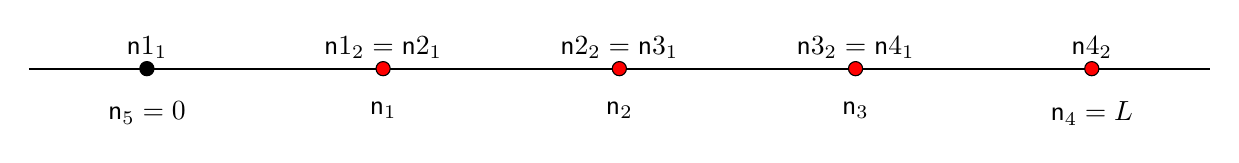
\begin{tikzpicture}[scale=3.0]
\draw[-,thick](-0.5,0) -- (4.5,0);
\draw[fill] (0,0) circle (0.03cm);
\foreach \x in {1, ..., 4}
    \draw[fill=red] (\x,0) circle (0.03cm);
\node[below] at (0,-0.1) {$\mathsf{n}_5=0$};
\node[below] at (1,-0.1) {$\mathsf{n}_1$};
\node[below] at (2,-0.1) {$\mathsf{n}_2$};
\node[below] at (3,-0.1) {$\mathsf{n}_3$};
\node[below] at (4,-0.1) {$\mathsf{n}_4=L$};
\node[above] at (0,0) {$\mathsf{n}\brak{1}_1$};
\node[above] at (1,0) {$\mathsf{n}\brak{1}_2=\mathsf{n}\brak{2}_1$};
\node[above] at (2,0) {$\mathsf{n}\brak{2}_2=\mathsf{n}\brak{3}_1$};
\node[above] at (3,0) {$\mathsf{n}\brak{3}_2=\mathsf{n}\brak{4}_1$};
\node[above] at (4,0) {$\mathsf{n}\brak{4}_2$};
\end{tikzpicture}
\end{center}
\end{figure}

\begin{example}\label{example: node numbers 1d}
If $P=4$ then
\[
\boldsymbol{T}=\begin{bmatrix}
5&1&2&3\\
1&2&3&4\end{bmatrix}.
\]
\end{example}

Writing $U\brak{p}_k=u_h(\mathsf{n}\brak{p}_k)$~and
$V\brak{p}_j=v(\mathsf{n}\brak{p}_j)$, we see that
\[
u_h(x)=\sum_{k=1}^2U\brak{p}_k\psi\brak{p}_k(x)
\quad\text{and}\quad
v(x)=\sum_{j=1}^2V\brak{p}_j\psi\brak{p}_j(x)
\quad\text{for $x\in[x_{p-1},x_p]$.}
\]
Thus,
\[
\int_0^Lf(x)v(x)\,dx=\sum_{p=1}^P\int_{x_{p-1}}^{x_p}f(x)\sum_{j=1}^2
    V\brak{p}_j\psi\brak{p}_j(x)\,dx
    =\sum_{p=1}^P\sum_{j=1}^2 f\brak{p}_jV_j\brak{p}
\]
and
\begin{align*}
\int_0^La(x)u_h'(x)v'(x)\,dx
    &=\sum_{p=1}^P\int_{x_{p-1}}^{x_p}a(x)
    \biggl(\sum_{k=1}^2 U\brak{p}_k(\psi_k\brak{p})'(s)\biggr)
    \biggl(\sum_{j=1}^2 V\brak{p}_j(\psi_j\brak{p})'(x)\biggr)\,dx\\
    &=\sum_{p=1}^P\sum_{k=1}^2\sum_{j=1}^2
    U\brak{p}_ka\brak{p}_{jk}V\brak{p}_j;
\end{align*}
likewise
\[
\int_0^Lc(x)u_h(x)v(x)\,dx=\sum_{p=1}^P\sum_{k=1}^2\sum_{j=1}^2
    U\brak{p}_kc\brak{p}_{jk}V\brak{p}_j
\quad\text{and}\quad
v(L)=V\brak{P}_2.
\]
Therefore, \eqref{eq: self-adjoint mixed bc FEM} holds iff
\[
\sum_{p=1}^P\sum_{j=1}^2V\brak{p}_j
\sum_{k=1}^2\bigl(a\brak{p}_{jk}+c\brak{p}_{jk}\bigr)U\brak{p}_k
    =\gamma_LV\brak{P}_2+\sum_{p=1}^P\sum_{j=1}^2V\brak{p}_jf\brak{p}_j
    \quad\text{for all $v\in T_h$.}
\]

For~$v\in V_h$, put
\[
V_r=v(\mathsf{n}\brak{p}_r)\quad\text{for $1\le r\le P+1$,}
\]
so that $V_r=V\brak{p}_j$ iff $r=t_{jp}$, and hence
\[
\sum_{p=1}^{P+1}\sum_{j=1}^2V\brak{p}_jf\brak{p}_j=\sum_{r=1}^PV_rf_r,
\]
where
\[
f_r=\sum_{j\in\mathcal{I}_r}f\brak{p}_j
\quad\text{and}\quad
\mathcal{I}_r=\{\,(p,j):t_{jp}=r\,\}.
\]
Similarly, put $U_s=u_h(\mathsf{n}_s)$ so that $U_s=U\brak{p}_k$ iff 
$s=t_{kp}$, and hence
\[
\sum_{p=1}^P\sum_{j=1}^2V\brak{p}_j\sum_{k=1}^2
\bigl(a\brak{p}_{jk}+c\brak{p}_{jk}\bigr)U\brak{p}_k
=\sum_{r=1}^{P+1}V_r\sum_{s=1}^{P+1}(a_{rs}+c_{rs})U_s
\]
where
\[
a_{rs}=\sum_{(p,j,k)\in\mathfrak{I}_{rs}}a\brak{p}_{jk}
\qquad\text{and}\qquad
c_{rs}=\sum_{(p,j,k)\in\mathfrak{I}_{rs}} c\brak{p}_{jk},
\]
with
\[
\mathcal{I}_{rs}=\{\,(p,j,k):\text{$t_{jp}=r$ and $t_{kp}=s$}\,\}.
\]
In this way, \eqref{eq: self-adjoint mixed bc FEM} holds iff
\[
\sum_{r=1}^PV_r\sum_{s=1}^{P+1}(a_{rs}+c_{rs})U_s=\gamma_LV_{P}
	+\sum_{r=1}^PV_r\sum_{s=1}^{P+1}(a_{rs}+c_{rs})U_s,
\]
remembering that $V_{P+1}=v(\mathsf{n}_{P+1})=v(0)=0$.  Forming the 
$P\times(P+1)$ matrices $\boldsymbol{A}=[a_{pq}]$~and 
$\boldsymbol{C}=[c_{pq}]$, and the $P$-dimensional vector~$\boldsymbol{f}$,
we see that
\begin{equation}\label{eq: VT(A+C)U}
\boldsymbol{V}^T\bigl(\boldsymbol{A}+\boldsymbol{C}\bigr)\boldsymbol{U}
    =\gamma_LV_P+\boldsymbol{V}^T\boldsymbol{f}
    \quad\text{for all $\boldsymbol{V}\in\mathbb{R}^P$,}
\end{equation}
and therefore
\begin{equation}\label{eq: A C f example}
\bigl(\boldsymbol{A}+\boldsymbol{C}\bigr)\boldsymbol{U}
    =\gamma_L\boldsymbol{e}_P+\boldsymbol{f}.
\end{equation}

Partition the matrices as
$\boldsymbol{A}=[\boldsymbol{A}\free\quad\boldsymbol{A}\fix]$~and
$\boldsymbol{C}=[\boldsymbol{C}\free\quad\boldsymbol{C}\fix]$, where
$\boldsymbol{A}\free$~and $\boldsymbol{C}\free$ are $P\times P$, and so
$\boldsymbol{A}\fix$~and $\boldsymbol{C}\fix$ are $P\times1$.  Likewise
partition the vector~$\boldsymbol{U}=[\boldsymbol{U}\free\quad U\fix]^T$ where
$\boldsymbol{U}\free$ is $P\times1$ and so $U\fix$ is $1\times1$, that is, a
scalar.  Since $U\fix=U_{P+1}=u_h(\mathsf{n}_{P+1})=u_h(0)=\gamma_0$,
\[
\bigl(\boldsymbol{A}+\boldsymbol{C}\bigr)\boldsymbol{U}
    =\bigl[(\boldsymbol{A}\free+\boldsymbol{C}\free)\quad
    (\boldsymbol{A}\fix+\boldsymbol{C}\fix)\bigr]
    \begin{bmatrix}\boldsymbol{U}\free\\ U\fix\end{bmatrix}
    =(\boldsymbol{A}\free+\boldsymbol{C}\free)\boldsymbol{U}\free
    +\gamma_0(\boldsymbol{A}\fix+\boldsymbol{C}\fix),
\]
yielding the $P\times P$ linear system
\begin{equation}\label{eq: FEM 1d mixed linear system}
\bigl(\boldsymbol{A}\free+\boldsymbol{C}\free\bigr)\boldsymbol{U}\free
=\boldsymbol{f}-\gamma_0(\boldsymbol{A}\fix+\boldsymbol{C}\fix)
    +\gamma_L\boldsymbol{e}_P.
\end{equation}
Algorithm~\ref{alg: assemble f piecewise linear} shows how, using the 
connectivity matrix~$\boldsymbol{T}=[t_{pm}]$, the global load 
vector~$\boldsymbol{f}$ can be assembled from the element load 
vectors~$\boldsymbol{f}\brak{p}$.  Likewise, 
algorithm~\ref{alg: assemble A piecewise linear} shows how the global 
stiffness matrix~$\boldsymbol{A}$ can be assembled from the element stiffness 
matrices~$\boldsymbol{A}\brak{p}$.  The global mass matrix~$\boldsymbol{C}$ is 
assembled in the same way. In practice, $\boldsymbol{A}$~and $\boldsymbol{C}$ 
are constructed an appropriate \emph{sparse matrix} data structure.

\begin{algorithm}
\caption{Assemble the load vector $\boldsymbol{f}$
from~\eqref{eq: A C f example}.}
\label{alg: assemble f piecewise linear}
\begin{algorithmic}
\State Allocate storage for $\boldsymbol{f}=[f_p]\in\mathbb{R}^P$.
\For{$p=1:P$}
    \State $f_p=0$
\EndFor
\For{$p=1:P$}
    \State Compute $\boldsymbol{f}\brak{p}$
    \For{$j=1:2$}
        \State $r=t_{pj}$\Comment{$\mathsf{n}_r=\mathsf{n}\brak{p}_j$}
        \If{$r\le M$}
            \State $f_r\gets f_r+f\brak{p}_j$
        \EndIf
    \EndFor
\EndFor
\end{algorithmic}
\end{algorithm}

\begin{algorithm}
\caption{Assemble the stiffness matrix $\boldsymbol{A}$
from~\eqref{eq: A C f example}.}
\label{alg: assemble A piecewise linear}
\begin{algorithmic}
\State Allocate storage for
$\boldsymbol{A}=[a_{pq}]\in\mathbb{R}^{P\times(P+1)}$
\For{$p=1:P$}
    \For{$q=1:P+1$}
        \State $a_{pq}=0$
    \EndFor
\EndFor
\For{$p=1:P$}
    \State Compute $\boldsymbol{A}\brak{p}$
    \For{$j=1:2$}
        \State $r=e_{jp}$
        \If{$r\le P$}
            \For{$k=1:2$}
                \State $s=t_{kp}$
                \State $a_{rs}\gets a_{rs}+a\brak{p}_{jk}$
            \EndFor
        \EndIf
    \EndFor
\EndFor
\end{algorithmic}
\end{algorithm}

\begin{example}\label{example: assemble A}
Let $L=4$ and consider a uniform grid with $P=4$ subintervals, and suppose 
that $a(x)=1=c(x)$.  Thus, by \cref{example: linear elt matrix 1d},
\[
h_p=1,\quad\boldsymbol{A}\brak{p}=\begin{bmatrix}1&-1\\ -1&1\end{bmatrix},\quad
\boldsymbol{C}=\frac{1}{6}\begin{bmatrix}2&1\\ 1&2\end{bmatrix},
\]
and by \cref{example: node numbers 1d},
\[
\mathcal{I}_1=\{(1,2),(2,1)\},\quad
\mathcal{I}_2=\{(2,2),(3,1)\},\quad
\mathcal{I}_3=\{(3,2),(4,1)\},\quad
\mathcal{I}_4=\{(4,2)\},
\]
so
\[
f_1=f\brak{1}_2+f\brak{2}_1,\quad
f_2=f\brak{2}_2+f\brak{3}_1,\quad
f_3=f\brak{3}_2+f\brak{4}_1,\quad
f_4=f\brak{4}_2.
\]
Furthermore,
\begin{align*}
\mathcal{I}_{11}&=\{(1,2,2),(2,1,1)\},&
\mathcal{I}_{12}&=\{(2,1,2)\},&
\mathcal{I}_{15}&=\{(1,2,1)\},\\
\mathcal{I}_{21}&=\{(2,2,1)\},&
\mathcal{I}_{22}&=\{(2,2,2),(3,1,1)\},&
\mathcal{I}_{23}&=\{(3,1,2)\},\\
\mathcal{I}_{32}&=\{(3,2,1)\},&
\mathcal{I}_{33}&=\{(3,2,2),(4,1,1)\},&
\mathcal{I}_{34}&=\{(4,1,2)\},\\
\mathcal{I}_{43}&=\{(4,2,1)\},&
\mathcal{I}_{44}&=\{(4,2,2)\},&&
\end{align*}
with $\mathcal{I}_{rs}=\emptyset$ otherwise, and hence
\begin{align*}
a_{11}&=a\brak{1}_{22}+a\brak{2}_{11},&
a_{12}&=a\brak{2}_{12},&
a_{15}&=a\brak{1}_{21},\\
a_{21}&=a\brak{2}_{21},&
a_{22}&=a\brak{2}_{22}+a\brak{3}_{11},&
a_{23}&=a\brak{3}_{12},\\
a_{32}&=a\brak{3}_{21},&
a_{33}&=a\brak{3}_{22}+a\brak{4}_{11},&
a_{34}&=a\brak{4}_{12},\\
a_{43}&=a\brak{4}_{21},&
a_{44}&=a\brak{4}_{22}.&&
\end{align*}
Assembling the $4\times5$ stiffness 
matrix~$\boldsymbol{A}=[\boldsymbol{A}\free\quad\boldsymbol{A}\fix]$ 
amounts to computing
\[
\left[
\begin{array}{cccc|c}1&0&0&0&-1\\0&0&0&0&0\\0&0&0&0&0\\0&0&0&0&0\end{array}
\right]+\left[
\begin{array}{cccc|c}1&-1&0&0&0\\-1&1&0&0&0\\0&0&0&0&0\\0&0&0&0&0\end{array}
\right]+\left[
\begin{array}{cccc|c}0&0&0&0&0\\0&1&-1&0&0\\0&-1&1&0&0\\0&0&0&0&0\end{array}
\right]+\left[
\begin{array}{cccc|c}0&0&0&0&0\\0&0&0&0&0\\0&0&1&-1&0\\0&0&-1&1&0\end{array}
\right],
\]
resulting in
\[
\boldsymbol{A}=\left[\begin{array}{cccc|c}
2&-1&0&0&-1\\ -1&2&-1&0&0\\ 0&-1&2&-1&0\\ 0&0&-1&1&0\end{array}\right],\qquad
\boldsymbol{A}\free=\begin{bmatrix}
2&-1&0&0\\ -1&2&-1&0\\ 0&-1&2&-1\\ 0&0&-1&1\end{bmatrix},\qquad
\boldsymbol{A}\fix=\begin{bmatrix}-1\\ 0\\ 0\\ 0\end{bmatrix}.
\]
Similarly, we find that the mass 
matrix~$\boldsymbol{C}=[\boldsymbol{C}\free\quad\boldsymbol{C}\fix]$ is given by
\[
\boldsymbol{C}=\frac{1}{6}\left[\begin{array}{cccc|c}
4&1&0&0&1\\ 1&4&1&0&0\\ 0&1&4&1&0\\ 0&0&1&2&0\end{array}\right],\qquad
\boldsymbol{C}\free=\frac{1}{6}\begin{bmatrix}
4&1&0&0\\ 1&4&1&0\\ 0&1&4&1\\ 0&0&1&2\end{bmatrix},\qquad
\boldsymbol{C}\fix=\frac{1}{6}\begin{bmatrix}1\\ 0\\ 0\\ 0\end{bmatrix}.
\]
\end{example}

\section{Quadratic elements}\label{sec: quadratic elements}

Let us again consider the self-adjoint, two-point boundary-value 
problem~\eqref{eq: self-adjoint mixed} but now let $V_h$ denote the vector 
space consisting of the continuous, piecewise-\emph{quadratic} functions with 
respect to the grid points~$x_p$.  Thus, a function~$v:[0,L]\to\mathbb{R}$ 
belongs to~$V_h$ iff there are polynomials $v_1$, $v_2$, \dots, $v_M$ of degree 
at most~$2$ such that \eqref{eq: v piecewise}~and \eqref{eq: v cts} hold.
For the $p$th element~$[x_{p-1},x_p]$, we now define three nodes
\[
\mathsf{n}\brak{p}_1=x_{p-1},\qquad
\mathsf{n}\brak{p}_2=\tfrac12(x_{p-1}+x_p),\qquad
\mathsf{n}\brak{p}_3=x_p.
\]
Notice that $\mathsf{n}\brak{p}_2$ is the midpoint of the element.
Corresponding to these nodes are the quadratic shape functions
\begin{equation}\label{eq: quadratic psi 1d}
\begin{aligned}
\psi\brak{p}_1(x)
	&=2h_p^{-2}(x-\mathsf{n}\brak{p}_2)(x-\mathsf{n}\brak{p}_3),\\
\psi\brak{p}_2(x)
	&=4h_p^{-2}(x-\mathsf{n}\brak{p}_1)(\mathsf{n}\brak{p}_3-x),\\
\psi\brak{p}_3(x)
	&=2h_p^{-2}(x-\mathsf{n}\brak{p}_1)(x-\mathsf{n}\brak{p}_2),
\end{aligned}
\end{equation}
and Exercise~\ref{ex: quadratic DoF 1d} shows that
\begin{equation}\label{eq: quadratic DoF 1d}
\psi\brak{p}_j(\mathsf{n}\brak{p}_k)=\delta_{jk}.
\end{equation}
The global enumeration of the free nodes is
\[
\mathsf{n}_{2p-1}=\tfrac12(x_{p-1}+x_p)
\quad\text{and}\quad
\mathsf{n}_{2p}=x_p\quad\text{for $1\le p\le P$,}
\]
and the fixed node is $\mathsf{n}_{2P+1}=x_0$.  The connectivity 
matrix~$\boldsymbol{T}=[t_{jp}]$ is now $3\times P$, with $t_{jp}$ again given 
by~\eqref{eq: e pm def}.  For example, if $P=6$ then 
\[
\boldsymbol{T}=\begin{bmatrix}
13&2&4&6&8&10\\
 1&3&5&7&9&11\\
 2&4&6&8&10&12          
\end{bmatrix}.
\]

We define the \emph{reference element}~$[0,1]$ with \emph{reference nodes}
\[
\mathsf{n}_1=0,\qquad\mathsf{n}_2=\frac{1}{2},\qquad\mathsf{n}_3=1,
\]
and corresponding quadratic (reference) shape functions
\begin{equation}\label{eq: quadratic shape funcs 1d}
\Psi_1(\xi)=2(\xi-\tfrac12)(\xi-1),\qquad
\Psi_2(\xi)=4\xi(1-\xi),\qquad
\Psi_3(\xi)=2\xi(\xi-\tfrac12),
\end{equation}
satisfying $\Psi_j(\mathsf{n}_k)=\delta_{jk}$ for $j$, $k\in\{1,2,3\}$.  
In this way,
\[
\Psi_j(\xi)=\psi\brak{p}_j(x)\quad
	\text{if $x=x_{p-1}+\xi h_p$,}\quad\text{for $0\le\xi\le1$,}
\]
and since $dx/d\xi=h_p$, the chain rule implies that
\[
\Psi'_j(\xi)=h_p(\psi\brak{p}_j)'(x).
\]
Thus, the entries of the $3\times3$ element stiffness 
matrix~$\boldsymbol{A}\brak{p}=[a_{jk}]$ are given by
\begin{equation}\label{eq: a reference 1d}
a\brak{p}_{jk}=\frac{1}{h_p}\int_0^1a(x_{p-1}+\xi h_p)
	\Psi'_k(\xi)\Psi'_j(\xi)\,d\xi,
\end{equation}
and those of the $3\times3$ element mass 
matrix~$\boldsymbol{C}=[c\brak{p}_{jk}]$ by
\begin{equation}\label{eq: c reference 1d}
c\brak{p}_{jk}=h_p\int_0^1c(x_{p-1}+\xi h_p)
	\Psi_k(\xi)\Psi_j(\xi)\,d\xi.
\end{equation}

\begin{example}\label{ex: quadratic Am Cm}
If $a(x)=1$~and $c(x)=1$, then
\begin{equation}\label{eq: element matrices quadratic 1d}
\boldsymbol{A}\brak{p}=\frac{1}{3h_p}\begin{bmatrix}
 7&-8& 1\\
-8&16&-8\\
 1&-8& 7\end{bmatrix}
\quad\text{and}\quad
\boldsymbol{C}\brak{p}=\frac{h_p}{30}\begin{bmatrix}
 4& 2&-1\\
 2&16& 2\\
-1& 2& 4 \end{bmatrix}
\end{equation}
\end{example}

To deal with non-constant coefficients $a(x)$~and $c(x)$, it is convenient to 
approximate the integrals \eqref{eq: a reference 1d}~and
\eqref{eq: c reference 1d} using a \emph{quadrature rule}
\[
\int_0^1 f(\xi)\,d\xi\approx\sum_{l=1}^J w_lf(\xi_l)
\]
with \emph{weights} $w_1$, $w_2$, \dots, $w_J$ and \emph{points}
\[
0\le\xi_1<\xi_2<\cdots<\xi_J\le1.
\]
Using such an approximation yields, for the element stiffness matrix,
\[
\boldsymbol{A}\brak{p}\approx
	\widetilde{\boldsymbol{A}}\brak{p}=[\tilde a_{jk}\brak{p}]
\quad\text{where}\quad
\tilde a\brak{p}_{jk}=\frac{1}{h_p}\sum_{j=1}^Jw_la(x_{p-1}+\xi_lh_p)
	\Psi'_k(\xi_l)\Psi'_j(\xi_l),
\]
and for the element mass matrix,
\[
\boldsymbol{C}\brak{p}\approx
	\widetilde{\boldsymbol{C}}\brak{p}=[\tilde c_{jk}\brak{p}]
\quad\text{where}\quad
\tilde c\brak{p}_{jk}=h_p\sum_{j=1}^Jw_lc(x_{p-1}+\xi_lh_p)
	\Psi_k(\xi_l)\Psi_j(\xi_l).
\]
With the help of the connectivity matrix~$\boldsymbol{T}$, the $3\times3$ 
element matrices $\boldsymbol{A}\brak{p}$~and $\boldsymbol{C}\brak{p}$ can be 
assembled into the $(2P)\times(2P+1)$ global matrices $\boldsymbol{A}$~and 
$\boldsymbol{C}$; see exercise~\ref{ex: assemble quadratic 1d}.

By adapting the arguments that led to~\eqref{eq: VT(A+C)U} we find that the 
vector~$\boldsymbol{U}=[U_j]_{j=1}^{2P+1}$ of nodal values 
$U_j=u_h(\mathsf{n}_j)$ satisfies
\[
\boldsymbol{V}^T(\boldsymbol{A}+\boldsymbol{C})\boldsymbol{U}
	=\gamma_LV_{2M}+\boldsymbol{V}^T\boldsymbol{f}
	\quad\text{for all $\boldsymbol{V}\in\mathbb{R}^{2P}$.}
\]
We again use the partitionings
\[
\boldsymbol{A}=[\boldsymbol{A}\free\quad\boldsymbol{A}\fix],\qquad
\boldsymbol{C}=[\boldsymbol{C}\free\quad\boldsymbol{C}\fix],\qquad
\boldsymbol{U}=[\boldsymbol{U}\free\quad U\fix]^T,
\]
but now $\boldsymbol{A}\free$~and $\boldsymbol{C}$ are $(2P)\times(2P)$, and
$\boldsymbol{A}\fix$, $\boldsymbol{C}\fix$ and $\boldsymbol{U}\free$ are 
$(2P)\times1$, with $U\fix=\gamma_0$.  It follows that $\boldsymbol{U}\free$ 
again satisfies a linear system of the 
form~\eqref{eq: FEM 1d mixed linear system}, but this system is now 
$(2P)\times(2P)$.

\section{Polynomial interpolation}

Let $\mathbb{P}_r$ denote the vector space of real polynomials of degree at 
most~$r$.  Let $x_1$, $x_2$, \dots, $x_{r+1}$ be distinct points in an 
interval~$[a,b]$, and let $f:[a,b]\to\mathbb{R}$ be a continuous function.  We 
say that a polynomial~$g\in\mathbb{P}_r$ \emph{interpolates} $f$ at the given 
points if
\begin{equation}\label{eq: g interpolates f}
g(x_j)=f(x_j)\quad\text{for $1\le j\le r+1$.}
\end{equation}
To see that such a $g$ exists, we define the \emph{Lagrange 
interpolation polynomials} $\ell_1$, $\ell_2$, \dots, $\ell_{r+1}$ by
\begin{equation}\label{eq: ell_j def}
\ell_j(x)=\prod_{1\le k\le r+1, k\ne j}
	\frac{x-x_k}{x_j-x_k}\quad\text{for $1\le j\le r+1$,}
\end{equation}
and then define the \emph{linear interpolation operator}~$\mathcal{Q}_r$ by
\[
(\mathcal{Q}_rf)(x)=\sum_{j=1}^{r+1}f(x_j)\ell_j(x).
\]
Observe that $\ell_j\in\mathbb{P}_r$ because it is the product of~$r$ linear 
factors.  Moreover, if $x=x_j$ then each factor in the 
product~\eqref{eq: ell_j def} equals~$1$ and so $\ell_j(x_j)=1$, whereas if 
$x=x_k$ for some~$k\ne j$, then one factor equals~$0$ and so $\ell_j(x_k)=0$.
In other words,
\[
\ell_j(x_k)=\delta_{jk}\quad\text{for $j$, $k\in\{1,2,\ldots,r+1\}$.}
\]
It follows that $\mathcal{Q}_rf\in\mathbb{P}_r$ interpolates~$f$, that is,
\[
(\mathcal{Q}_rf)(x_j)=f(x_j)\quad\text{for $1\le j\le r+1$.}
\]
Furthermore, $\mathcal{Q}_rf$ is the only such interpolant, because if 
$g\in\mathbb{P}_r$ satisfies \eqref{eq: g interpolates f} then the difference
$g-\mathcal{Q}_rf$ is a polynomial satisfying
\[
(g-\mathcal{Q}_rf)(x_j)=g(x_j)-(\mathcal{Q}_rf)(x_j)=f(x_j)-f(x_j)=0
	\quad\text{for $1\le j\le r+1$,}
\]
so, for some constant~$C$,
\[
g(x)-(\mathcal{Q}_rf)(x)=C(x-x_1)(x-x_2)\cdots(x-x_{r+1}) 
	=Cx^{r+1}+\text{lower degree terms}.
\]
But $g-\mathcal{Q}_rf$ has degree at most~$r$, so $C=0$ and hence
$g(x)=(\mathcal{Q}_rf)(x)$ for all~$x$. In particular, since any element 
of~$\mathbb{P}_r$ interpolates itself, it follows that
\[
\mathcal{Q}_rf=f\quad\text{for every $f\in\mathbb{P}_r$,}
\]
and thus $\mathcal{Q}_r^2=\mathcal{Q}_r$.  Hence, $\mathcal{Q}_r$ is a 
\emph{projection} onto~$\mathbb{P}_r$.

Let 
\begin{equation}\label{eq: pi r y}
\pi_{r,y}(x)=\frac{(x-y)_+^r}{r!}=\begin{cases}
	(x-y)^r/r!&\text{if $a\le y\le x\le b$,}\\
	0&\text{if $a\le x<y\le b$.}
\end{cases}
\end{equation}
If $f$ is $C^{r+1}$ on~$[a,b]$ then, by Theorem~\ref{thm: Taylor remainder}, 
\[
f(x)=\sum_{k=0}^r\frac{f^{(k)}(a)}{k!}\,(x-a)^k
	+\int_a^b\pi_{r,y}(x)f^{(r+1)}(y)\,dy\quad\text{for $a\le x\le b$.}
\]
Since the sum on the right defines a function in~$\mathbb{P}_r$,
applying $\mathcal{Q}_r$ to both sides gives
\[
(\mathcal{Q}_rf)(x)=\sum_{k=0}^r\frac{f^{(k)}(a)}{k!}\,(x-a)^k
	+\int_a^b(\mathcal{Q}_r\pi_{r,y})(x)f^{(r+1)}(y)\,dy
\quad\text{for $a\le x\le b$.}
\]
Hence, the \emph{interpolation error} has the integral representation
\begin{equation}\label{eq: Qr f error}
(\mathcal{Q}_rf)(x)-f(x)=\int_a^b K_r(x,y)f^{(r+1)}(y)\,dy
\quad\text{for $a\le x\le b$,}
\end{equation}
where the \emph{Peano kernel} is defined by
\[
K_r(x,y)=(\mathcal{Q}_r\pi_{r,y})(x)-\pi_{r,y}(x)
	\quad\text{for $x$, $y\in[a,b]$.}
\]

\begin{figure}
\caption{Peano kernel for linear interpolation at $0$~and $1$
(Example~\ref{example: linear interp}.}
\label{fig: linear Peano}
\begin{center}
\includegraphics[scale=0.6]{../src/chap2/Linear_PeanoK_3d.pdf}
\includegraphics[scale=0.5]{../src/chap2/Linear_PeanoK_contour.pdf}
\end{center}
\end{figure}

\begin{example}\label{example: linear interp}
Consider \emph{linear interpolation}, that is, $r=1$, with interpolation points 
$x_1=a$~and $x_2=b$.  In this case, the Lagrange polynomials are
\[
\ell_1(x)=\frac{x-x_2}{x_1-x_2}=\frac{b-x}{b-a}
\quad\text{and}\quad
\ell_2(x)=\frac{x-x_1}{x_2-x_1}=\frac{x-a}{b-a},
\]
and
\[
(\mathcal{Q}_1f)(x)=f(a)\ell_1(x)+f(b)\ell_2(x)
	=f(a)\,\frac{b-x}{b-a}+f(b)\,\frac{x-a}{b-a}.
\]
In particular, since $\pi_{1,y}(a)=0$~and $\pi_{1,y}(b)=b-y$ for~$a\le y\le b$,
\[
(\mathcal{Q}_1\pi_{1,y})(x)=\pi_{1,y}(a)\ell_1(x)+\pi_{1,y}(b)\ell_2(x)
	=\frac{(b-y)(x-a)}{b-a}\quad\text{for $x$, $y\in[a,b]$,}
\]
so
\[
K_1(x,y)=\frac{(b-y)(x-a)}{b-a}-(x-y)\quad\text{for $a\le y\le x\le b$,}
\]
and
\[
K_1(x,y)=\frac{(b-y)(x-a)}{b-a}\quad\text{for $a\le x\le y\le b$.}
\]
Thus, $K_1(x,y)$ is piecewise linear in~$x$ for fixed~$y$, and vice versa, with
\[
K_1(a,y)=0=K_1(b,y),\qquad K_1(x,a)=0=K_1(x,b),\qquad
K_1(x,x)=\frac{(b-x)(x-a)}{b-a}.
\]
\end{example}

\begin{figure}
\caption{Peano kernel~\eqref{eq: quadratic Peano} for quadratic interpolation 
at $-1$, $0$~and $+1$.}\label{fig: quadratic Peano}
\begin{center}
\includegraphics[scale=0.6]{../src/chap2/Quadratic_PeanoK_3d.pdf}
\includegraphics[scale=0.5]{../src/chap2/Quadratic_PeanoK_contour.pdf}
\end{center}
\end{figure}

\begin{example}\label{example: quadratic interp}
Let $x_1=-1$, $x_2=0$~and $x_3=1$.  The quadratic Lagrange polynomials are
\[
\ell_1(x)=\frac{(x-0)(x-1)}{(-1-0)(-1-1)},\qquad
\ell_2(x)=\frac{(x+1)(x-1)}{(0+1)(0-1)},\qquad
\ell_3(x)=\frac{(x+1)(x-0)}{(1+1)(1-0)},
\]
that is,
\[
\ell_1(x)=\tfrac12x(x-1),\qquad
\ell_2(x)=(1+x)(1-x),\qquad
\ell_3(x)=\tfrac12x(x+1).
\]
Since $\pi_{2,y}(-1)=0$, $\pi_{2,y}(0)=\tfrac12(-y)_+^2$~and 
$\pi_{2,y}(1)=\tfrac12(1-y)^2$ for~$-1\le y\le 1$,
\begin{equation}\label{eq: quadratic Peano}
K_2(x,y)=\tfrac12(-y)_+^2\ell_2(x)+\tfrac12(1-y)^2\ell_3(x)-\tfrac12(x-y)_+^2.
\end{equation}
Observe that $\ell_1(-x)=\ell_3(x)$ and $\ell_2(-x)=\ell_2(x)$, so
\[
K_2(-x,-y)=\tfrac12(y)_+^2\ell_2(x)+\tfrac12(1+y)^2\ell_1(x)-\tfrac12(y-x)_+^2
\]
and thus
\[
K_2(x,y)+K_2(-x,-y)=\tfrac12y^2\ell_2(x)+\tfrac12(1-y)^2\ell_3(x)
	+\tfrac12(1+y)^2\ell_1(x)-\tfrac12(x-y)^2.
\]
We use the identity $\ell_1(x)+\ell_2(x)+\ell_3(x)=(\mathcal{Q}_21)(x)=1$ to
replace $\ell_2(x)$ with~$1-\ell_1(x)-\ell_3(x)$ and deduce that
\begin{align*}
K_2(x,y)+K_2(-x,-y)&=\tfrac12\bigl[y^2-(x-y)^2\bigr]
	+\tfrac12\bigl[(1+y)^2-y^2\bigr]\ell_1(x)
	+\tfrac12\bigl[(1-y)^2-y^2\bigr]\ell_3(x)\\
	&=\tfrac12x(2y-x)+\tfrac12(1+2y)\ell_1(x)+\tfrac12(1-2y)\ell_3(x)\\
	&=\tfrac12\bigl[\ell_1(x)+\ell_3(x)-x^2\bigr]
	+y\bigl[x+\ell_3(x)-\ell_1(x)\bigr]=0.
\end{align*}
Hence, $K_2$ possesses the symmetry property (Figure~\ref{fig: quadratic Peano})
\begin{equation}\label{eq: K2 symmetry}
K_2(-x,-y)=-K_2(x,y)\quad\text{for $x$, $y\in[-1,1]$.}
\end{equation}
\end{example}

Since the $j$th derivative~$\pi_{r,y}^{(j)}(x)=\pi_{r-j,y}(x)$, we see that
\[
\partial_x^jK_r(x,y)=(\mathcal{Q}_r\pi_{r,y})^{(j)}(x)-\pi_{r-j,y}(x)
\quad\text{for $0\le j\le r$,}
\]
and that the $j$th derivative of the interpolation error has the representation
\begin{equation}\label{eq: Qr f error deriv}
(\mathcal{Q}_rf-f)^{(j)}(x)=\int_a^b\partial_x^j K_r(x,y)f^{(r+1)}(y)\,dy
\quad\text{for $a\le x\le b$.}
\end{equation}


\section{Accuracy of piecewise-polynomial approximation}
\label{sec: accuracy of interpolation}

Fix $r+1$~nodes in the reference element~$[0,1]$,
\begin{equation}\label{eq: ref nodes 1d}
0=\mathsf{n}_1<\mathsf{n}_2<\cdots<\mathsf{n}_{r+1}=1,
\end{equation}
and consider an element~$[x_{p-1},x_p]$ with length~$h_p=x_p-x_{p-1}$.  The 
change of variable,
\[
x = x_{p-1} + \xi h_p\quad\text{for $\xi\in[0,1]$,}
\]
defines an affine bijection~$\xi\mapsto x$ from the reference element~$[0,1]$ 
onto~$[x_{p-1},x_p]$.  We assume that the nodes in~$[x_{p-1},x_p]$ correspond 
to the reference nodes under this affine bijection, that is,
\[
\mathsf{n}_j\brak{p}=x_{p-1}+\mathsf{n}_jh_p\quad\text{for $1\le j\le r+1$.}
\]
Given a function $f(x)$, we define $\hat f$ on the reference element by
\[
\hat f(\xi)=f(x)\quad\text{where $x=x_{p-1}+\xi h_p$,}
\]
and let $\mathcal{Q}_r\brak{p}$~and $\widehat{\mathcal{Q}}_r$ denote 
polynomial interpolation operators for $[x_{p-1},x_p]$~and $[0,1]$, 
respectively, so that
\[
\mathcal{Q}_r\brak{p}f\in\mathbb{P}_{r+1}\quad\text{and}\quad
(\mathcal{Q}_r\brak{p}f)(\mathsf{n}_j\brak{p})=f(\mathsf{n}_j\brak{p})
\quad\text{for $1\le j\le r+1$,}
\]
whereas
\[
\widehat{\mathcal{Q}}_r\hat f\in\mathbb{P}_{r+1}\quad\text{and}\quad
\bigl(\widehat{\mathcal{Q}}_r\hat f\bigr)(\mathsf{n}_j)=\hat f(\mathsf{n}_j)
\quad\text{for $1\le j\le r+1$.}
\]
Notice that if we let $g(x)=(\mathcal{Q}_r\brak{p}f)(x)$, then 
$\hat g(\xi)=\widehat{\mathcal{Q}}_r\hat f(\xi)$ because 
$\hat g\in\mathbb{P}_r$~and 
\[
\hat g(\mathsf{n}_j)=g(\mathsf{n}_j\brak{p})=f(\mathsf{n}_j\brak{p})
    =\hat f(\mathsf{n}_j)\quad\text{for $1\le j\le r+1$.}
\]
In other words, 
$\widehat{\mathcal{Q}_r\brak{p}f}=\widehat{\mathcal{Q}}_r\hat f$.

\begin{theorem}
Assume that $f$ is $C^{r+1}$ on~$[x_{p-1},x_p]$, and let $K_r$ denote the Peano 
kernel for polynomial interpolation at the $r+1$~nodes of the reference 
element~$[0,1]$.  Then,
\[
\int_{x_{p-1}}^{x_p}|(f-\mathcal{Q}_r\brak{p}f)^{(k)}(x)|^2\,dx
    \le C_{r,k}h_p^{2(r+1-k)}\int_{x_{p-1}}^{x_p}|\hat f^{(r+1)}(x)|^2\,dx
    \quad\text{for $0\le k\le r$,}
\]
where the constant
\[
C_{r,k}=\int_0^1\int_0^1|\partial_\xi^kK_r(\xi,\eta)|^2\,d\eta\,d\xi
\]
depends only on $k$~and the choice of the $r+1$ nodes~\eqref{eq: ref nodes 1d}.
\end{theorem}
\begin{proof}
Since $dx/d\xi=h_p$ we see that
\[
\hat f^{(k)}(\xi)=h_p^k f^{(k)}(x),
\]
so using \eqref{eq: Qr f error deriv} and the Cauchy--Schwarz inequality,
\begin{align*}
\bigl|(f-\mathcal{Q}_r\brak{p}f)^{(k)}(x)\bigr|^2
    &=h_p^{-2k}\bigl|\bigl(\hat f-\widehat{Q}_r\hat f)(\xi)\bigr|^2
    =h_p^{-2k}\biggl|\int_0^1\partial_\xi^k K_r(\xi,\eta)
        \hat f^{(r+1)}(\eta)\, d\eta\biggr|^2\\
    &\le h_p^{-2k}\biggl(\int_0^1|\partial_\xi^kK_r(\xi,\eta)|^2\,d\eta\biggr)
    \biggl(\int_0^1|\hat f^{(r+1)}(\eta)|^2\,d\eta\biggr)
\end{align*}
for $0\le\xi\le1$.  Integrating with respect to~$x$, and noting that 
$dx=h_p\,d\xi$, we have
\begin{align*}
\int_{x_{p-1}}^{x_p}\bigl|(f-\mathcal{Q}_rf)^{(k)}(x)\bigr|^2\,dx
&=h_p^{1-2k}\int_0^1\bigl|\bigl(\hat f-\widehat{Q}_r\hat f)(\xi)\bigr|^2\,d\xi\\
&\le h_p^{1-2k}\biggl(
    \int_0^1\int_0^1|\partial_\xi^kK_r(\xi,\eta)|^2\,d\eta\,d\xi\biggr)
    \biggl(\int_0^1|\hat f^{(r+1)}(\eta)|^2\,d\eta\biggr),
\end{align*}
and 
\[
\int_0^1|\hat f^{(r+1)}(\eta)|^2\,d\eta=\int_{x_{p-1}}^{x_p}
    |h_p^{r+1}f^{(r+1)}(y)|^2h_p^{-1}\,dy,
\]
which implies the desired estimate.
\end{proof}

For any continuous~$v:[0,L]\to\mathbb{R}$ we define $\mathcal{Q}_{r,h}v$, the 
\emph{piecewise-polynomial interpolant} of degree at most~$r$, by
\[
(\mathcal{Q}_{r,h}v)(x)
    =(\mathcal{Q}_r\brak{p}v)(x)\quad\text{for $x\in[x_{p-1},x_p]$;}
\]
since $\mathsf{n}\brak{p-1}_{r+1}=x_{p-1}=\mathsf{n}\brak{p}_1$ we see 
that
\[
(\mathcal{Q}_r\brak{p-1}v)(x_{p-1})=v(x_{p-1})
    =(\mathcal{Q}_r\brak{p}v)(x_{p-1})\quad\text{for~$2\le p\le P-1$,}
\]
and hence the function~$\mathcal{Q}_{r,h}v$ is continuous on~$[0,L]$.

\begin{theorem}\label{thm: Q r h}
If $v$ is $C^{r+1}$ on~$[0,L]$, then
\[
\|v-\mathcal{Q}_{r,h}v\|_{L_2(0,L)}
    \le\sqrt{C_{r,0}}\,h^{r+1}\|v^{(r+1)}\|_{L_2(0,L)}
\]
and
\[
\|v'-(\mathcal{Q}_{r,h}v)'\|_{L_2(0,L)}
    \le\sqrt{C_{r,1}}\,h^r\|v^{(r+1)}\|_{L_2(0,L)}.
\]
\end{theorem}
\begin{proof}
We have
\begin{align*}
\|v-\mathcal{Q}_{r,h}v\|_{L_2(0,L)}^2
    &=\int_0^L|(v-\mathcal{Q}_{r,h}v)(x)|^2\,dx=\sum_{p=1}^P
    \int_{x_{p-1}}^{x_p}|(v-\mathcal{Q}_r\brak{p}v)(x)|^2\,dx\\
    &\le\sum_{p=1}^P C_{r,0}h_p^{2(r+1)}\int_{x_{p-1}}^{x_p}
        |\hat v^{(r+1)}(x)|^2\,dx\\
    &\le C_{r,0}h^{2(r+1)}\sum_{p=1}^M\int_{x_{p-1}}^{x_p} 
        |\hat v^{(r+1)}(x)|^2\,dx
    =C_{r,0}h^{2(r+1)}\|v^{(r+1)}\|_{L_2(0,L)}^2,
\end{align*}
which proves the first estimate.  The second follows in the same way.
\end{proof}

\section{Optimality property}
Subtracting \eqref{eq: <u,v>A} from~\eqref{eq: <uh,v>A}, we see that the
error~$e_h=u_h-u$ in the finite element solution is energy-orthogonal to the 
test space~$T_h$, that is, 
\begin{equation}\label{eq: energy orthog}
\iprod{e_h,v}_{\mathcal{L}}=0\quad\text{for all $v\in T_h$.}
\end{equation}
Using this property, we show in the next theorem that $u_h$ is the best 
approximation to~$u$ by a function in the trial space~$S_h$, as measured by 
the energy norm.

\begin{theorem}\label{thm: optimality}
The finite element solution~$u_h\in S_h$ satisfies
\[
\|u_h-u\|_{\mathcal{L}}\le\|w-u\|_{\mathcal{A}}
	\quad\text{for all $w\in S_h$.}
\]
\end{theorem}
\begin{proof}
Let $w\in S_h$ and observe that the error~$e_h=u_h-u$ satisfies
\begin{align*}
\|e_h\|_{\mathcal{L}}^2=\iprod{e_h,e_h}_{\mathcal{A}}
	&=\iprod{e_h,u_h-u}_{\mathcal{L}}
	=\iprod{e_h,u_h-w+w-u}_{\mathcal{L}}\\
	&=\iprod{e_h,u_h-w}_{\mathcal{L}}+\iprod{e_h,w-u}_{\mathcal{A}}.
\end{align*}
Since $(u_h-w)(0)=u_h(0)-w(0)=\gamma_0-\gamma_0=0$ we see that $u_h-w\in T_h$
and so the energy-orthogonality property~\eqref{eq: energy orthog} implies
that $\iprod{e_h,u_h-w}_{\mathcal{L}}=0$.  Hence, by the Cauchy--Schwarz
inequality,
\[
\|e_h\|_{\mathcal{L}}^2=\iprod{e_h,w-u}_{\mathcal{A}}
	\le\|e_h\|_{\mathcal{L}}\|w-u\|_{\mathcal{A}},
\]
which implies the desired inequality.
\end{proof}

By combining \cref{thm: optimality} with the approximation property of the 
interpolant~$\mathcal{Q}_{r,h}u$ proved in \cref{thm: Q r h}, we can show
that the finite element error, measured in the energy norm, is $O(h^r)$.

\begin{theorem}\label{thm: uh-u L}
Assume that the solution~$u:[0,L]\to\mathbb{R}$ of the boundary-value 
problem~\eqref{eq: self-adjoint mixed} is~$C^{r+1}$.  Then,
there is a constant~$C>0$, independent of~$h$, such that
\[
\|u_h-u\|_{\mathcal{L}}\le Ch^r\|u^{(r+1)}\|.
\]
\end{theorem}
\begin{proof}
Let $w=\mathcal{Q}_{r,h}u$.  Since $w(0)=u(0)=\gamma_0$ we see that $w\in S_h$,
so we may apply \cref{thm: optimality} and deduce that
\begin{align*}
\|u_h-u\|_{\mathcal{L}}^2\le\|w-u\|_{\mathcal{A}}^2
	&\le a_{\max}\|w'-u'\|^2+c_{\max}\|w-u\|^2\\
	&\le\bigl(a_{\max}C_{r,1}h^{2r}+c_{\max}C_{r,0}h^{2r+2}\bigr)
	\|u^{(r+1)}\|^2\\
	&=\bigl(a_{\max}C_{r,1}+c_{\max}C_{r,0}h^2\bigr)
	\bigl(h^r\|v^{(r+1)}\|\bigr)^2,
\end{align*}
which implies the result since $h$ is bounded.
\end{proof}
\begin{corollary}
$\|u_h'-u'\|\le Ch^r\|u^{(r+1)}\|$.
\end{corollary}
\begin{proof}
Observe that since $a(x)/a_{\min}\ge1$,
\[
\|v'\|^2=\int_0^L|v'(x)|^2\,dx\le\int_0^L\frac{a(x)}{a_{min}}\,|v'(x)|^2\,dx
	=\frac{1}{a_{\min}}\int_0^La(x)|v'(x)|^2\,dx
	\le\frac{\|v\|_{\mathcal{L}}^2}{a_{\min}},
\]
and in particular $\|u_h'-u'\|^2\le\|u_h-u\|^2_{\mathcal{L}}/a_{min}$.
\end{proof}

In some applications, an integral of the form
\[
\iprod{\phi,u}=\int_0^L\phi(x)u(x)\,dx
\]
is of interest.  The next theorem shows that if $\phi\in H^r(0,L)$~and 
$u\in H^{r+1}(0,L)$, then
\[
\iprod{\phi,u_h}=\iprod{\phi,u}+O(h^{2r+1}).
\]

\begin{theorem}
If $0\le k\le r$, then
\[
|\iprod{u_h-u,\phi}|\le Ch^{k+1}\|\phi\|_{H^k(0,L)}\|u_h-u\|_{\mathcal{L}}.
\]
\end{theorem}
\begin{proof}
Given $\phi$, let $\theta$ be the solution of the boundary-value problem
\[
\mathcal{L}\theta=\phi(x)\quad\text{for $0<x<L$,}
	\quad\text{with $\theta(0)=0$ and $a(L)\theta'(L)=0$,}
\]
so that
\[
\iprod{\theta,v}_{\mathcal{L}}=\iprod{\phi,v}\quad\text{whenever $v(0)=0$.}
\]
Since $(u_h-u)(0)=u_h(0)-u(0)=\gamma_0-\gamma_0=0$, it follows that
\[
\iprod{\phi,u_h-u}=\iprod{\theta,u_h-u}_{\mathcal{L}}
	=\iprod{\theta-Q_{k+1,h}\theta,u_h-u}_{\mathcal{L}},
\]
where, in the second step, we used the fact that $u_h-u$ is energy-orthogonal
to $Q_{k+1,h}\theta\in T_h$ because $k\le r$.  Hence, by the Cauchy--Schwarz 
inequality,
\[
|\iprod{\phi,u_h-u}|\le\|\theta-Q_{k+1,h}\theta\|_{\mathcal{L}}
	\|u_h-u\|_{\mathcal{L}}.
\]
Since
\[
\|\theta-\mathcal{Q}_{k+1,h}\theta\|_{\mathcal{L}}^2
	\le a_{\max}\|\theta'-(\mathcal{Q}_{k+1,h}\theta)'\|
	+c_{\max}\|\theta-\mathcal{Q}_{k+1,h}\theta\|
	\le C\bigl(h^{k+1}+h^{k+2})\|\theta^{(k+2)}\|
\]
it suffices to show, using induction on~$k$, that 
$\|\theta^{(k+2)}\|\le C\|\phi\|_{H^k(0,L)}$.  
Rearranging the ODE $a\theta''+c\theta=\phi$,  and using \cref{lem: v v'} 
followed by~\cref{thm: ||u||A},
\[
\|\theta''\|=\|(\phi-c\theta)/a\|
	\le\frac{\|\phi\|+c_{\max}\|\theta\|}{a_{\min}}\le C\|\phi\|
	\le C(\|\phi\|+\|\theta\|_{\mathcal{L}})\le C\|\phi\|,
\]
which proves the claim for~$k=0$.  For the inductive step, we let~$k\ge1$ and
assume that 
\[
\|\theta^{(j+2)}\|\le C\sum_{l=0}^j\|\phi^{(l)}\|
	\quad\text{for~$0\le j\le k-1$.}
\]
By $k$-fold differentiation of $a\theta''+c\theta=\phi$, 
\[
a\theta^{(k+2)}+c\theta^{(k)}+\sum_{j=0}^{k-1}\binom{k}{j}\bigl(
	a^{(k-j)}\theta^{(j+2)}+c^{(k-j)}\theta^{(j)}\bigr)=\phi^{(k)}
\]
so
\[
\theta^{(k)}=\frac{1}{a}\bigg(\phi^{(k)}-c\theta^{(k)}
	-\sum_{j=0}^{k-1}\binom{k}{j}\bigl(
	a^{(k-j)}\theta^{(j+2)}+c^{(k-j)}\theta^{(j)}\bigr)\biggr)
\]
and
\[
\|\theta^{(k)}\|\le C\biggl(\|\phi^{(k)}\|+\|\theta\|+\|\theta'\|
	+\sum_{j=2}^{k+1}\|\theta^{(j)}\|\biggr)
\le C\biggl(\|\phi^{(k)}\|+\|\theta\|_{\mathcal{L}}
	+\sum_{j=0}^{k-1}\|\theta^{(j+2)}\|\biggr),
\]
implying that the induction goes through.
\end{proof}

\begin{corollary}
$\|u_h-u\|\le Ch^{r+1}\|u^{(r+1)}\|$.
\end{corollary}
\begin{proof}
Apply \cref{thm: uh-u L} with $\phi=u_h-u$~and $k=0$ to obtain
\[
\|u_h-u\|^2=\iprod{u_h-u,u_h-u}\le Ch\|u_h-u\|\|u_h-u\|_{\mathcal{L}}
	\le Ch\|u_h-u\|h^r\|u^{(r+1)}\|,
\]
which implies the result.
\end{proof}

\section{Sturm--Liouville problems}\label{sec: Sturm-Liouville}

We will now consider a Sturm--Liouville equation,
\begin{equation}\label{eq: Sturm Liouville ODE}
-\bigl(a(x)\phi'\bigr)'+\bigl(c(x)-\lambda b(x)\bigr)\phi=0\quad
	\text{for $0<x<L$,}
\end{equation}
subject to (homogeneous) mixed boundary conditions
\begin{equation}\label{eq: Sturm Liouville bc}
\phi(0)=0\quad\text{and}\quad a(L)\phi'(L)=0.
\end{equation}
In addition to assuming that the leading coefficient~$a(x)$ 
satisfies~\eqref{eq: ellipticity 1d}, we require that
\begin{equation}\label{eq: b>0}
b(x)>0\quad\text{for $0<x<L$.}
\end{equation}
A non-trivial solution~$\phi=\phi(x)$ is said to an \emph{eigenfunction} and 
$\lambda$ is then the corresponding \emph{eigenvalue}.  

The ODE~\eqref{eq: Sturm Liouville ODE} can be written as
\[
\mathcal{L}\phi=\lambda b\phi,
\]
where the self-adjoint differential operator~$\mathcal{L}$ is again given 
by~\eqref{eq: L self-adjoint}.  Recalling the 
identity~\eqref{eq: Lu v by parts}, we see that any \emph{eigenpair} 
$(\phi,\lambda)$ satisfies, for any test function~$v$,
\[
\int_0^L\bigl(a(x)\phi'(x)v(x)+c(x)\phi(x)v(x)\bigr)\,dx
	=\lambda\int_0^Lb(x)\phi(x)v(x)\,dx
\quad\text{provided $v(0)=0$.}
\]

Let $V_h$ denote the continuous, piecewise-quadratic finite element space 
discussed in Section~\ref{sec: quadratic elements}, and put
\[
S_h=T_h=\{\,v\in V_h:v(0)=0\,\}.
\]
We seek an approximate eigenfunction~$\phi_h\in S_h$ and corresponding 
approximate eigenvalue~$\lambda_h$ such that
\[
\int_0^L\bigl(a(x)\phi_h'(x)v(x)+c(x)\phi_h(x)v(x)\bigr)\,dx
	=\lambda\int_0^Lb(x)\phi_h(x)v(x)\,dx
\quad\text{for all $v\in T_h$.}
\]
Let $\chi_1$, $\chi_2$, \dots, $\chi_{2P+1}$ be the nodal basis for~$V_h$, so 
that
\[
\chi_r(\mathsf{n}_s)=\delta_{rs}
	\quad\text{for $r$, $s\in\{1,2,\ldots, 2P+1\}$,}
\]
and thus, since $\phi_h(\mathsf{n}_{2P+1})=\phi_h(x_0)=\phi_h(0)=0$,
\[
\phi_h(x)=\sum_{s=1}^{2P}\Phi_s\chi_s(x)
	\quad\text{for $0\le x\le L$},
	\quad\text{where $\Phi_s=\phi_h(\mathsf{n}_s)$.}
\]
Choosing $v=\chi_r$ we see that
\[
\sum_{k=1}^{2P}\bigl(a_{rs}+c_{rs}\bigr)\Phi_s
	=\lambda_h\sum_{s=1}^{2P}b_{rs}\Phi_s\quad\text{for $1\le r\le 2P$,}
\]
where
\[
a_{rs}=\int_0^La(x)\chi'_s(x)\chi'_r(x)\,dx,\qquad
c_{rs}=\int_0^Lc(x)\chi_s(x)\chi_r(x)\,dx,
\]
and
\[
b_{rs}=\int_0^Lb(x)\chi_s(x)\chi_r(x)\,dx.
\]
In this way, we obtain a $(2P)\times(2P)$ \emph{generalised algebraic 
eigenproblem},
\[
\bigl(\boldsymbol{A}+\boldsymbol{C}\bigr)\boldsymbol{\Phi}
	=\Lambda\boldsymbol{B}\boldsymbol{\Phi},
\]
where $\boldsymbol{A}=[a_{rs}]_{r,s=1}^{2P}$, 
$\boldsymbol{C}=[c_{rs}]_{r,s=1}^{2P}$, 
$\boldsymbol{B}=[b_{rs}]_{r,s=1}^{2P}$, 
$\boldsymbol{\Phi}=[\Phi_s]_{s=1}^{2P}$~and 
$\Lambda=\lambda_h$.  Each of the three matrices is real and symmetric, and our 
assumptions \eqref{eq: ellipticity 1d}~and \eqref{eq: b>0} on the coefficients 
$a(x)$~and $b(x)$ ensure that $\boldsymbol{A}$~and $\boldsymbol{B}$ are 
strictly positive-definite.  It follows that there exist eigenpairs 
$(\Phi_s,\Lambda_s)$ for~$1\le s\le 2P$, with
\[
\Lambda_1\le\Lambda_2\le\cdots\le\Lambda_{2P},\qquad
\boldsymbol{\Phi}_r^T(\boldsymbol{A}+\boldsymbol{C})
    \boldsymbol{\Phi}_s=\Lambda_s\delta_{rs},\qquad
\boldsymbol{\Phi}_r^T\boldsymbol{B}\boldsymbol{\Phi}_s=\delta_{rs}.
\]
For a practical implementation, it is simpler to assemble $\boldsymbol{A}$, 
$\boldsymbol{B}$~and $\boldsymbol{C}$ from the corresponding element matrices
$\boldsymbol{A}\brak{p}$, $\boldsymbol{B}\brak{p}$~and 
$\boldsymbol{C}\brak{p}$; see Exercise \ref{ex: assemble quadratic 1d}~(iii).

\begin{Exercises}

\exercise\label{ex: V_h vector space}
Prove that the set~$V_h$ of continuous, piecewise-linear functions is a vector 
space.

\exercise
Show that the trial set~\eqref{eq: Sh 1D} is a \emph{convex subset} of~$V_h$,
that is, if $v$, $w\in S_h$ then $\lambda v+\mu w\in S_h$ for all $\lambda\ge0$
and $\mu\ge$ such that $\lambda+\mu=1$.

\exercise
Prove that $\{\chi_p\}_{p=0}^P$ is a basis for~$V_h$, and that 
$\{\chi_p\}_{p=1}^{P-1}$ is a basis for~$T_h$.

\exercise
Consider the model problem~\eqref{eq: model 1d chap 2}.  Define a uniform 
mesh~$x_p=ph$ on~$[0,L]$ for $0\le p\le P=M$ where $h=\Delta x=L/P$.  Denote 
the finite difference solution by~$U^{\mathrm{d}}_p\approx u(x_p)$, and denote 
the nodal values of the piecewise-linear finite element solution 
by~$U^{\mathrm{e}}_p=u_h(x_p)\approx u(x_p)$.  Let 
\[
f^{\,\mathrm{d}}_p=f(x_p)\quad\text{and}\quad
f^{\,\mathrm{e}}_p=\frac{1}{h}\int_{x_{p-1}}^{x_{p+1}}f(x)\chi_p(x)\,dx
\quad\text{for $1\le p\le P-1$,}
\]
where $\chi_p$ is the $p$th piecewise-linear nodal basis function (that is, the 
``hat function'' centred on~$x_p$).  Let
\[
\boldsymbol{A}=\frac{1}{h^2}\begin{bmatrix}
 2&-1&      &      &      &\\
-1& 2&    -1&      &      &\\
  &  &\ddots&\ddots&\ddots&\\
  &  &      &    -1&     2&-1\\
  &  &      &      &    -1& 2
\end{bmatrix},\quad
\boldsymbol{f}^{\,\mathrm{d}}=\begin{bmatrix}
f^{\,\mathrm{d}}_1\\                              
f^{\,\mathrm{d}}_2\\                              
\vdots\\
f^{\,\mathrm{d}}_{P-2}\\                              
f^{\,\mathrm{d}}_{P-1}                              
\end{bmatrix},\quad
\boldsymbol{g}=\frac{1}{h^2}\begin{bmatrix}
\gamma_0\\ 0\\ \vdots\\ 0\\ \gamma_L                            
\end{bmatrix},
\]
so that $\boldsymbol{A}\boldsymbol{U}^{\mathrm{d}}=\boldsymbol{f}^{\,\mathrm{d}}
+\boldsymbol{g}$ as in~\eqref{eq: model 1d linear system}.
\begin{description}
\item{(i)} Show that $\boldsymbol{A}\boldsymbol{U}^{\mathrm{e}}
=\boldsymbol{f}^{\,\mathrm{e}}+\boldsymbol{g}$.
\item{(ii)} By applying Theorem~\ref{thm: discrete apriori 1D} to the finite 
difference equation satisfied by $U^{\mathrm{e}}_p-U^{\mathrm{d}}_p$, deduce 
that
\[
\max_{0\le p\le P}\bigl|U^{\mathrm{e}}_p-U^{\mathrm{d}}_p\bigr|
    \le\frac{L^2}{8}\,\max_{1\le p\le P-1}
    \bigl|f^{\,\mathrm{e}}_p-f^{\,\mathrm{d}}_p\bigr|.
\]
\item{(iii)}
Let $\delta_pf=f^{\,\mathrm{e}}_p-f^{\,\mathrm{d}}_p$, and
verify that $\delta_pf=0$ for all $f\in\mathbb{P}_1$.
(Hint: consider $f(x)=1$ and $f(x)=x-x_p$.)
\item{(iv)}
By applying $\delta_p$ to the Taylor expansion
\[
f(x)=f(x_{p-1})+f'(x_{p-1})(x-x_{p-1})+\int_{x_{p-1}}^x
	(x-y)f''(y)\,dy,
\]
show that 
\[
\delta_pf=\int_{x_{p-1}}^{x_{p+1}} K_p(y)f''(y)\,dy
\]
where, using the notation~\eqref{eq: pi r y},
\[
K_p(y)=\delta_p\pi_{1,y}=\frac{1}{6h^2}\times\begin{cases}
        (y-x_{p-1})^3,&x_{p-1}<y<x_p,\\
        (x_{p+1}-y)^3,&x_p<y<x_{p+1}.
\end{cases}
\]
\item{(v)}
Deduce using the Integral Mean Value Theorem that
\[
f^{\,\mathrm{e}}_p-f^{\,\mathrm{d}}_p=\frac{h^2}{12}\,f''(\xi)
\quad\text{for some $\xi\in[x_{p-1},x_{p+1}]$,}
\]
and hence conclude that the finite difference and finite element solutions 
agree to~$O(h^2)$.
\end{description}

\exercise
Consider a differential operator $\mathcal{L}u=-(au')'+bu'+cu$.  The term in 
$u'$ means that $\mathcal{L}$ is not self-adjoint (assuming $b$ is not 
identically zero), and the weak formulation of the mixed boundary-value 
problem~\eqref{eq: self-adjoint mixed} changes from~\eqref{eq: Lu=f weak 1d} to
\[
\int_0^L\bigl(au'v'+bu'v+cuv\bigr)\,dx
    =\gamma_Lv(L)+\int_0^Lfv\,dx\quad\text{provided $v(0)=0$,}
\]
with $u(0)=\gamma_0$, and the linear 
system~\eqref{eq: self-adjoint mixed equations} is now of the form
\[
\bigl(\boldsymbol{A}+\boldsymbol{B}+\boldsymbol{C}\bigr)\boldsymbol{U}
    =\boldsymbol{f}+\boldsymbol{g}.
\]
\begin{description}
\item{(i)} Why does the energy inner product no longer make sense.
\item{(ii)} How are the entries $b_{pq}$ of the matrix~$\boldsymbol{B}$ defined 
in terms of the nodal basis functions~$\phi_p$?
\item{(iii)} Assume now that $b(x)\equiv1$ and we use piecewise-linear elements.
\begin{description}
\item{(a)} Show that 
$b_{pq}+b_{qp}=\delta_{Pq}\delta_{Pp}-\delta_{0q}\delta_{0p}$.
\item{(b)} Hence find the diagonal entries $b_{pp}$ for $1\le p\le P$, and
the off-diagonal entries $b_{p,p-1}$~and $b_{p-1,p}$ for $2\le p\le P$.
\item{(c)} Write out $\boldsymbol{B}$ in the case $P=5$.
\end{description}
\end{description}
\begin{ans}
(ii) $b_{pq}=\int_0^Lb(x)\phi_q'(x)\phi_p(x)\,dx$\\
(iii) (b) $b_{00}=-1/2$, $b_{pp}=0$ for~$1\le p\le P-1$, $b_{PP}=1/2$\\
$b_{p,p-1}=-1/2$ and $b_{p-1,p}=1/2$ for $1\le p\le P$
(c) $\boldsymbol{B}=\frac{1}{2}\begin{bmatrix}
 0& 1& 0& 0&0\\
-1& 0& 1& 0&0\\
 0&-1& 0& 1&0\\
 0& 0&-1& 0&1\\
 0& 0& 0&-1&1\end{bmatrix}$
\end{ans}


\exercise
Check that the energy inner product~\eqref{eq: energy iprod} is in fact an 
inner product on the vector space of $C^1$ functions $v:[0,L]\to\mathbb{R}$ 
satisfying $v(0)=0$, by checking that for all such functions
\begin{description}
\item{(i)} $\iprod{v,w}_{\mathcal{L}}$ is linear in~$v$ for fixed $w$, and
vice versa.
\item{(ii)} $\iprod{v,w}_{\mathcal{L}}=\iprod{w,v}_{\mathcal{L}}$.
\item{(iii)} $\iprod{v,v}_{\mathcal{L}}\ge0$.
\item{(iv)} If $\iprod{v,v}_{\mathcal{L}}=0$ then $v\equiv0$.
\end{description}

\exercise\label{ex: quadratic DoF 1d}
Verify that the quadratic shape functions~\eqref{eq: quadratic psi 1d} on the 
$p$th element~$[x_{p-1},x_p]$ satisfy \eqref{eq: quadratic DoF 1d}.

\exercise
Recall the formulae \eqref{eq: a reference 1d}~and
\eqref{eq: c reference 1d} for the element stiffness and mass matrices using 
the quadratic shape functions~\eqref{eq: quadratic shape funcs 1d} on the 
reference element~$[0,1]$.  Assume that $a(x)=1$ and $c(x)=1$.
\begin{description}
\item{(i)} Verify that $\Psi_3(1-\xi)=\Psi_1(\xi)$ and 
$\Psi_2(1-\xi)=\Psi_2(\xi)$.
\item{(ii)} Deduce that
$a\brak{p}_{11}=a\brak{p}_{33}$, $a\brak{p}_{12}=a\brak{p}_{32}$,
$c\brak{p}_{11}=c\brak{p}_{33}$, $c\brak{p}_{12}=c\brak{p}_{32}$.
\item{(iii)} Verify the formulae \eqref{eq: element matrices quadratic 1d}
for the element stiffness and mass matrices.
\end{description}

\begin{figure}
\caption{The Peano kernel $K(y)$ for the quadrature rule of 
Exercise~\ref{ex: quadrature kernel}.}\label{fig: quadrature kernel}
\begin{center}
\includegraphics[scale=0.5]{../src/chap2/quadrature_kernel.pdf}
\end{center}
\end{figure}

\exercise\label{ex: quadrature kernel}
Consider a quadrature rule of the form
\[
\int_{-1}^1f(x)\,dx\approx w_1f(-1)+w_2f(-a)+w_2f(a)+w_1f(1)
\quad\text{with $0<a<1$,}
\]
and denote the error by
\[
Ef=\int_{-1}^1f(x)\,dx-\bigl(w_1f(-1)+w_2f(-a)+w_2f(a)+w_1f(1)\bigr).
\]
\begin{description}
\item{(i)} Why does $Ef=0$ if $f$ is an odd function, that is, if
$f(-x)=-f(x)$?
\item{(ii)} Simplify $Ef$ in the case when $f$ is an even function, that is, 
when $f(-x)=f(x)$. \item{(iii)}
Determine the values of $w_1$, $w_2$~and $a$ for which $Ef=0$ whenever
$f\in\mathbb{P}_5$.
\item{(iv)}
Deduce that there is a Peano kernel~$K$ such that, if $f$ is $C^6$ 
on~$[-1,1]$, then the rule given by part~(iii) has the error formula
\[
Ef=\int_{-1}^1K(y)f^{(6)}(y)\,dy.
\]
Express $K(y)$ in terms of the function $\pi_{5,y}(x)$ defined as 
in~\eqref{eq: pi r y}.
\item{(v)}
Write a script to verify that the graph of~$K$ is as shown in 
Figure~\ref{fig: quadrature kernel}.
\item{(vi)}
By considering the function~$f(x)=x^6$, show that 
\[
\int_{-1}^1K(y)\,dy=\frac{-32}{525}.
\]
\item{(vii)}
Hence determine the constant~$c$ such that, given a $C^6$ function~$f$,
there is a $\xi\in[-1,1]$ for which $Ef=cf^{(6)}(\xi)$.
\end{description}
\begin{ans}
(i) both sides equal $0$\quad (ii) $\int_0^1f(x)\,dx=w_1f(1)+w_2f(a)$\\
(iii) $a=1/\sqrt{5}$, $w_1=1/6$, $w_2=5/6$.\\
(iv) $K(y)=\pi_{6,y}(1)-\bigl(w_2\pi_{5,y}(-a)+w_2\pi_{5,y}(a)
+w_1\pi_{5,y}(1) \bigr)$\\
(vi) $c=\dfrac{-32}{6!\times525}=\dfrac{-2}{23,625}$.
\end{ans}

\exercise
Repeat the steps of Exercise~\ref{ex: quadrature kernel} for a quadrature rule
of the form
\[
\int_{-1}^1 f(x)\,dx\approx w_1f(-a)+w_2f(0)+w_1f(a).
\]
\begin{ans}
$w_1=5/9$, $w_2=8/9$, $a=\sqrt{3/5}$.
\end{ans}


\exercise\label{ex: assemble quadratic 1d}
Consider the two-point boundary-value problem~\eqref{eq: self-adjoint mixed} 
where $\mathcal{L}$ is of the form~\eqref{eq: L self-adjoint}, and let
\[
L=2,\qquad a(x)=1,\qquad c(x)=0,\qquad f(x)=18.
\]
\begin{description}
\item{(i)} Suppose we take a uniform mesh with~$M=6$ subintervals and apply the 
finite element method using quadratic elements.  Write down the connectivity 
matrix~$\boldsymbol{T}=[t_{jp}]$, the stiffness matrix~$\boldsymbol{A}$ and 
the load vector~$\boldsymbol{f}$. Hint: adapt the approach used in 
Example~\ref{example: assemble A} for piecewise-linear elements.
\item{(ii)} How do the boundary data $\gamma_0$~and $\gamma_L$ enter into the 
linear system for the nodal vector?
\item{(iii)} Formulate an algorithm to assemble the stiffness matrix for a 
general~$P$.  Hint: adapt Algorithm~\ref{alg: assemble A piecewise linear}.
\end{description}
\begin{ans}
(i) 
\begin{gather*}
\boldsymbol{T}=\begin{bmatrix}
13& 2& 4& 6& 8&10\\
 1& 3& 5& 7& 9&11\\
 2& 4& 6& 8&10&12
\end{bmatrix},\\
\boldsymbol{A}=\left[\begin{array}{cccccccccccc|c}
16&-8&  &  &  &  &  &  &  &  &  &  &-8\\
-8&14&-8& 1&  &  &  &  &  &  &  &  & 1\\
  &-8&16&-8&  &  &  &  &  &  &  &  &  \\
  & 1&-8&14&-8& 1&  &  &  &  &  &  &  \\
  &  &  &-8&16&-8&  &  &  &  &  &  &\\
  &  &  & 1&-8&14&-8& 1&  &  &  &  &  \\
  &  &  &  &  &-8&16&-8&  &  &  &  &  \\
  &  &  &  &  & 1&-8&14&-8& 1&  &  &  \\
  &  &  &  &  &  &  &-8&16&-8&  &  &  \\
  &  &  &  &  &  &  & 1&-8&14&-8& 1&  \\
  &  &  &  &  &  &  &  &  &-8&16&-8&  \\
  &  &  &  &  &  &  &  &  & 1&-8& 7&
\end{array}\right],\quad
\boldsymbol{f}=\left[\begin{array}{c}
4\\ 2\\ 4\\ 2\\ 4\\ 2\\ 4\\ 2\\ 4\\ 2\\ 4\\ 1
\end{array}\right].
\end{gather*}
(ii) $\boldsymbol{A}'\boldsymbol{U}'=\boldsymbol{f}-\gamma_0\boldsymbol{A}''
+\gamma_L\boldsymbol{e}_{2M}$\\
(iii)
\begin{algorithmic}
\State Allocate storage for 
$\boldsymbol{A}=[a_{jk}]\in\mathbb{R}^{(2M)\times(2M+1)}$ 
\For{$r=1:2P$}
    \For{$s=1:2P+1$}
        \State $a_{rs}=0$ 
    \EndFor
\EndFor
\For{$p=1:P$}
    \State Compute $\boldsymbol{A}\brak{p}$ 
    \For{$j=1:3$}
        \State $r=e_{jp}$
        \If{$r\le2P$}
            \For{$k=1:3$}
                \State $s=t_{kp}$
                \State $a_{rs}\gets a_{rs}+a\brak{p}_{jk}$
            \EndFor
        \EndIf
    \EndFor
\EndFor
\end{algorithmic}
\end{ans}

\exercise
Show that the Peano kernel for linear interpolation, discussed in 
Example~\ref{example: linear interp}, satisfies
\[
\int_a^b K_1(x,y)\,dy=\frac{1}{2}\,(x-a)(b-x)\quad\text{for $a\le x\le b$.}
\]
Hence use the integral mean value theorem to show that if~$f$ is $C^2$ 
on~$[a,b]$, then 
\[
(\mathcal{Q}_1f)(x)-f(x)=\frac{f''(\xi)}{2}\,(x-a)(b-x)
\]
for some~$\xi\in[a,b]$ (depending on~$x$).

\exercise
Let $x_1=-1$, $x_2=0$~and $x_3=+1$ as in 
Example~\ref{example: quadratic interp}.  
\begin{description}
\item{(i)} Show that if $g(x)=f(-x)$, then 
$(\mathcal{Q}_2g)(x)=(\mathcal{Q}_2f)(-x)$.
\item{(ii)} Deduce that if $f$ is $C^3$ on~$[-1,1]$, then
\[
\int_{-1}^1K_2(-x,y)f'''(y)\,dy=\int_{-1}^1K_2(x,y)g'''(y)\,dy
	\quad\text{for $-1\le x\le 1$.}
\]
\item{(iii)} Hence show that $K_2(-x,y)=-K_2(x,-y)$, in agreement 
with~\eqref{eq: K2 symmetry}.
\end{description}

\exercise
Sketch the graphs of the piecewise-quadratic nodal basis functions $\chi_1$, 
$\chi_2$, \dots, $\chi_{2P+1}$ used in section~\ref{sec: Sturm-Liouville}
for the case~$P=4$.

\exercise
Let $x_1=-1$, $x_2=0$, $x_3=1$, $x_4=2$ and consider the 
function~$f(x)=|x|$.
\begin{description}
\item{(i)} Find the corresponding Lagrange interpolation polynomials 
$\ell_1(x)$, $\ell_2(x)$, $\ell_3(x)$ and $\ell_4(x)$.
\item{(ii)} Hence write down $\mathcal{I}_3f$, the cubic interpolant to~$f$.
\end{description}
\begin{ans}
(i) $\ell_1(x)=-\tfrac16 x(x-1)(x-2)$, $\ell_2(x)=\tfrac12(x+1)(x-1)(x-2)$,
$\ell_3(x)=-\tfrac12(x+1)x(x-2)$, $\ell_4(x)=\tfrac16(x+1)x(x-1)$.\quad
(ii) $(\mathcal{I}_3f)(x)=\ell_1(x)+\ell_3(x)+2\ell_4(x)$
\end{ans}


\end{Exercises}
